% 'draft' mode can be used to speed up compilation
\documentclass[final]{hcmut-report}
% The report uses listings for commands and does not require minted.
\usepackage{listings}

% Full T5 (Vietnamese) glyph coverage
\usepackage{lmodern}

% Draft watermark
% https://github.com/callegar/LaTeX-draftwatermark

% Encodings
\usepackage{textcomp}

% Better tables
% Wide tables go to https://tex.stackexchange.com/q/332902
\usepackage{array,longtable,tabularx}

% Better enum
\usepackage{enumitem}

% Graphics
\usepackage{caption,float}

% References
% Use \Cref{} instead of \ref{}
\usepackage[nameinlink]{cleveref}

% Sub-preambles
% https://github.com/MartinScharrer/standalone

% Configurations
\coursename{Software Architecture (CO5185)}
% \reporttype{Report}
\title{VinaBeef RFID-based Livestock Farm Management System - Group 2}
\advisor{& Truong Thi Thai Minh &}
\stuname{%
  & Phan Ho Duy Thong & 2570775 \\
  & Nguyen Huu Phuc & 2352938 \\
  & Le Tran Khanh & 2570769 \\
  & Dang The Dong A & 2570791 \\
  & Nguyen Duc Phu & 2570772 \\
}

% Allow page breaks inside align* environment
%\allowdisplaybreaks{}

% Makes a lot of things blue, avoid at all costs
%\everymath{\color{blue}}

% Set depth of numbering for counters
\AtBeginDocument{\counterwithin{lstlisting}{section}}

% Rename some sections
%\AtBeginDocument{\renewcommand*{\contentsname}{Contents}}
%\AtBeginDocument{\renewcommand*{\refname}{References}}
%\AtBeginDocument{\renewcommand*{\bibname}{References}}

% Custom commands
%\newcommand*\mean[1]{\bar{#1}}

\begin{document}
\nocite{rabbitmq,pgAsyncCommit,rfc9110,awsRetries,owaspAuthz,owaspLogging,awsOutbox,seiQAW,c4model,richardsStyles,nygardADR,ibmActors}
\coverpage%

%\section*{Member list \& Workload}
%\newcounter{memberrowno}
%\setcounter{memberrowno}{0}
%\begin{center}
%  \begin{tabular}{>{\stepcounter{memberrowno}\thememberrowno}llcc}
%    \toprule
%    \multicolumn{1}{c}{\textbf{No.}} & \textbf{Full name} & \textbf{Student ID} & \textbf{Contribution} \\
%    \midrule
%                                     & h                  & xxxxxxx             & 100\%                       \\
%                                     & h                  & xxxxxxx             & 100\%                       \\
%    \bottomrule
%  \end{tabular}
%\end{center}
\clearpage

\tableofcontents
% \listoffigures
% \listoftables
% \lstlistoflistings{}

\clearpage
% \section{Normal section}
% This is how you normally work with \LaTeX, but you can also split a project into smaller files for easier management.
% To import other files, you can use \mintinline{latex}{\input{}} or \mintinline{latex}{\include{}}.
% There differences can be found at \url{https://tex.stackexchange.com/a/250}, but in short

% \begin{center}
%   \mintinline{latex}{\include{filename}} = \mintinline{latex}{\clearpage \input{filename} \clearpage}
% \end{center}

% \section{Label prefixes}
% There are no definite rules for label prefixes, but you can use the following as a guideline.
% \begin{itemize}
%   \item \textbf{chap:} for chapters
%   \item \textbf{sec:} for sections
%   \item \textbf{subsec:} for subsections
%   \item \textbf{eq:} for equations
%   \item \textbf{fig:} for figures
%   \item \textbf{tab:} for tables
%   \item \textbf{enum:} for enumerators and items
%   \item \textbf{fn:} for footnotes
%   \item \textbf{lst:} for listings
%   \item \textbf{alg:} for algorithms
%   \item \textbf{app:} for appendices
% \end{itemize}

% The \mintinline{latex}{\caption} macro increases the used counter and sets the current label text which is used by \mintinline{latex}{\label}.
% If you use \mintinline{latex}{\label} before it the old label text is used instead, which leads to a wrong number.
% Always use \mintinline{latex}{\label} after \mintinline{latex}{\caption} and not before or in it.

% That said, conventions are just conventions, and you can use whatever you want as long as you are consistent.

% \clearpage

% \input{chapters/example/better-tables.tex}
% \input{chapters/example/better-enum.tex}
% \include{chapters/example/codespace.tex}
% \include{chapters/example/figwidth.tex}

\section{System Context}\label{sec:1}

\subsection{Business Context}\label{sec:1.1}

VinaBeef Livestock Joint Stock Company operates large-scale beef cattle
farms in Dak Lak, Gia Lai and Dong Nai, with a standing herd of
approximately 25,000 cattle across 120 barns. Every animal wears a
unique RFID ear tag that serves as its permanent identifier for its
whole life on the farm.

Each barn has RFID gate readers at its entrances and exits. When cattle
pass through a gate, for example leaving for grazing or returning to the
barn, the reader records the animal' s identity and the
timestamp as a movement transaction, without manual work.

\subsection{Problem Statement}\label{sec:1.2}

\begin{itemize}
\item
  Manual head counts at this herd size are slow and error-prone, which delays the detection of missing or stray cattle.
\item
  Vaccination, treatment and movement records kept in separate places prevent a complete history for each animal.
\item
  Manual reporting to the National Animal Disease Control System delays disease surveillance; the assignment requires this exchange to use an API.
\item
  Management needs consolidated monitoring across the three farms, with data
  freshness and provisional/offline states visible.
\end{itemize}

These problems are derived from the assignment description, which does
not document VinaBeef's current manual process in detail.

\subsection{Objectives}\label{sec:1.3}

{\small
\begin{longtable}[]{|>{\raggedright\arraybackslash}p{\dimexpr 0.0753\linewidth-2\tabcolsep\relax}|>{\raggedright\arraybackslash}p{\dimexpr 0.4299\linewidth-2\tabcolsep\relax}|>{\raggedright\arraybackslash}p{\dimexpr 0.4649\linewidth-2\tabcolsep\relax}|}
\hline
\textbf{ID} & \textbf{Objective} & \textbf{Measure} \\ \hline
\endhead
\textbf{O1} & Automate movement recording at barn gates & 100\% of gate
passages recorded without manual input \\ \hline
\textbf{O2} & Detect abnormal situations quickly & Missing/unexpected
animals alerted within the configured window \\ \hline
\textbf{O3} & Keep a complete lifetime profile per animal & Vaccination,
health, treatment and movement history in one place \\ \hline
\textbf{O4} & Support regulatory health surveillance & Required data
sent to the National system through its API \\ \hline
\textbf{O5} & Ensure security and accountability & Role-based access;
every change audited \\ \hline
\end{longtable}
}

\subsection{Scope}\label{sec:1.4}

\textbf{In scope:} cattle and RFID tag management; barn, gate and reader
management; automated in/out movement recording and counting;
abnormality detection and alerting; vaccination, health and movement
history; reporting and auditing; system administration.

\textbf{Out of scope (this phase):} feed and nutrition management; sales
and slaughter traceability. The system manages only live-animal
identification, movement and health data within the farms.

\subsection{Assumptions and Constraints}\label{sec:1.5}

\begin{itemize}
\item
  Every animal is tagged with a unique, readable RFID ear tag before
  entering the system.
\item
  Farms are in rural areas; internet connectivity to the central site
  can be slow or interrupted.
\item
  Each gate has reader hardware able to determine passing direction (for
  example, two antennas or a reader pair).
\item
  The National Animal Disease Control System exposes an API for
  submitting outbreak and health surveillance data.
\item
  Peak load: about 200 cattle pass the gates of one farm within 30
  minutes during herd release or return.
\end{itemize}

\subsection{Stakeholders and Actors}\label{sec:1.6}

{\small
\begin{longtable}[]{|>{\raggedright\arraybackslash}p{\dimexpr 0.2794\linewidth-2\tabcolsep\relax}|>{\raggedright\arraybackslash}p{\dimexpr 0.1719\linewidth-2\tabcolsep\relax}|>{\raggedright\arraybackslash}p{\dimexpr 0.5187\linewidth-2\tabcolsep\relax}|}
\hline
\textbf{Actor} & \textbf{Type} & \textbf{Main goals} \\ \hline
\endhead
\textbf{Barn Supervisor} & Primary & Monitor head count, respond to
alerts, record health events in their barns \\ \hline
\textbf{Farm Manager} & Primary & Oversee all barns of a farm, manage
transfers, review reports \\ \hline
\textbf{System Administrator} & Primary & Manage users, roles, devices
and configuration \\ \hline
\textbf{Executive Management} & Primary & Monitor dashboards and
company-wide reports \\ \hline
\textbf{RFID Gate Reader} & System actor & Send tag read events
automatically \\ \hline
\textbf{National Animal Disease Control System} & External system &
Receive outbreak and health surveillance data \\ \hline
\end{longtable}
}

\begin{figure}[htbp]\centering
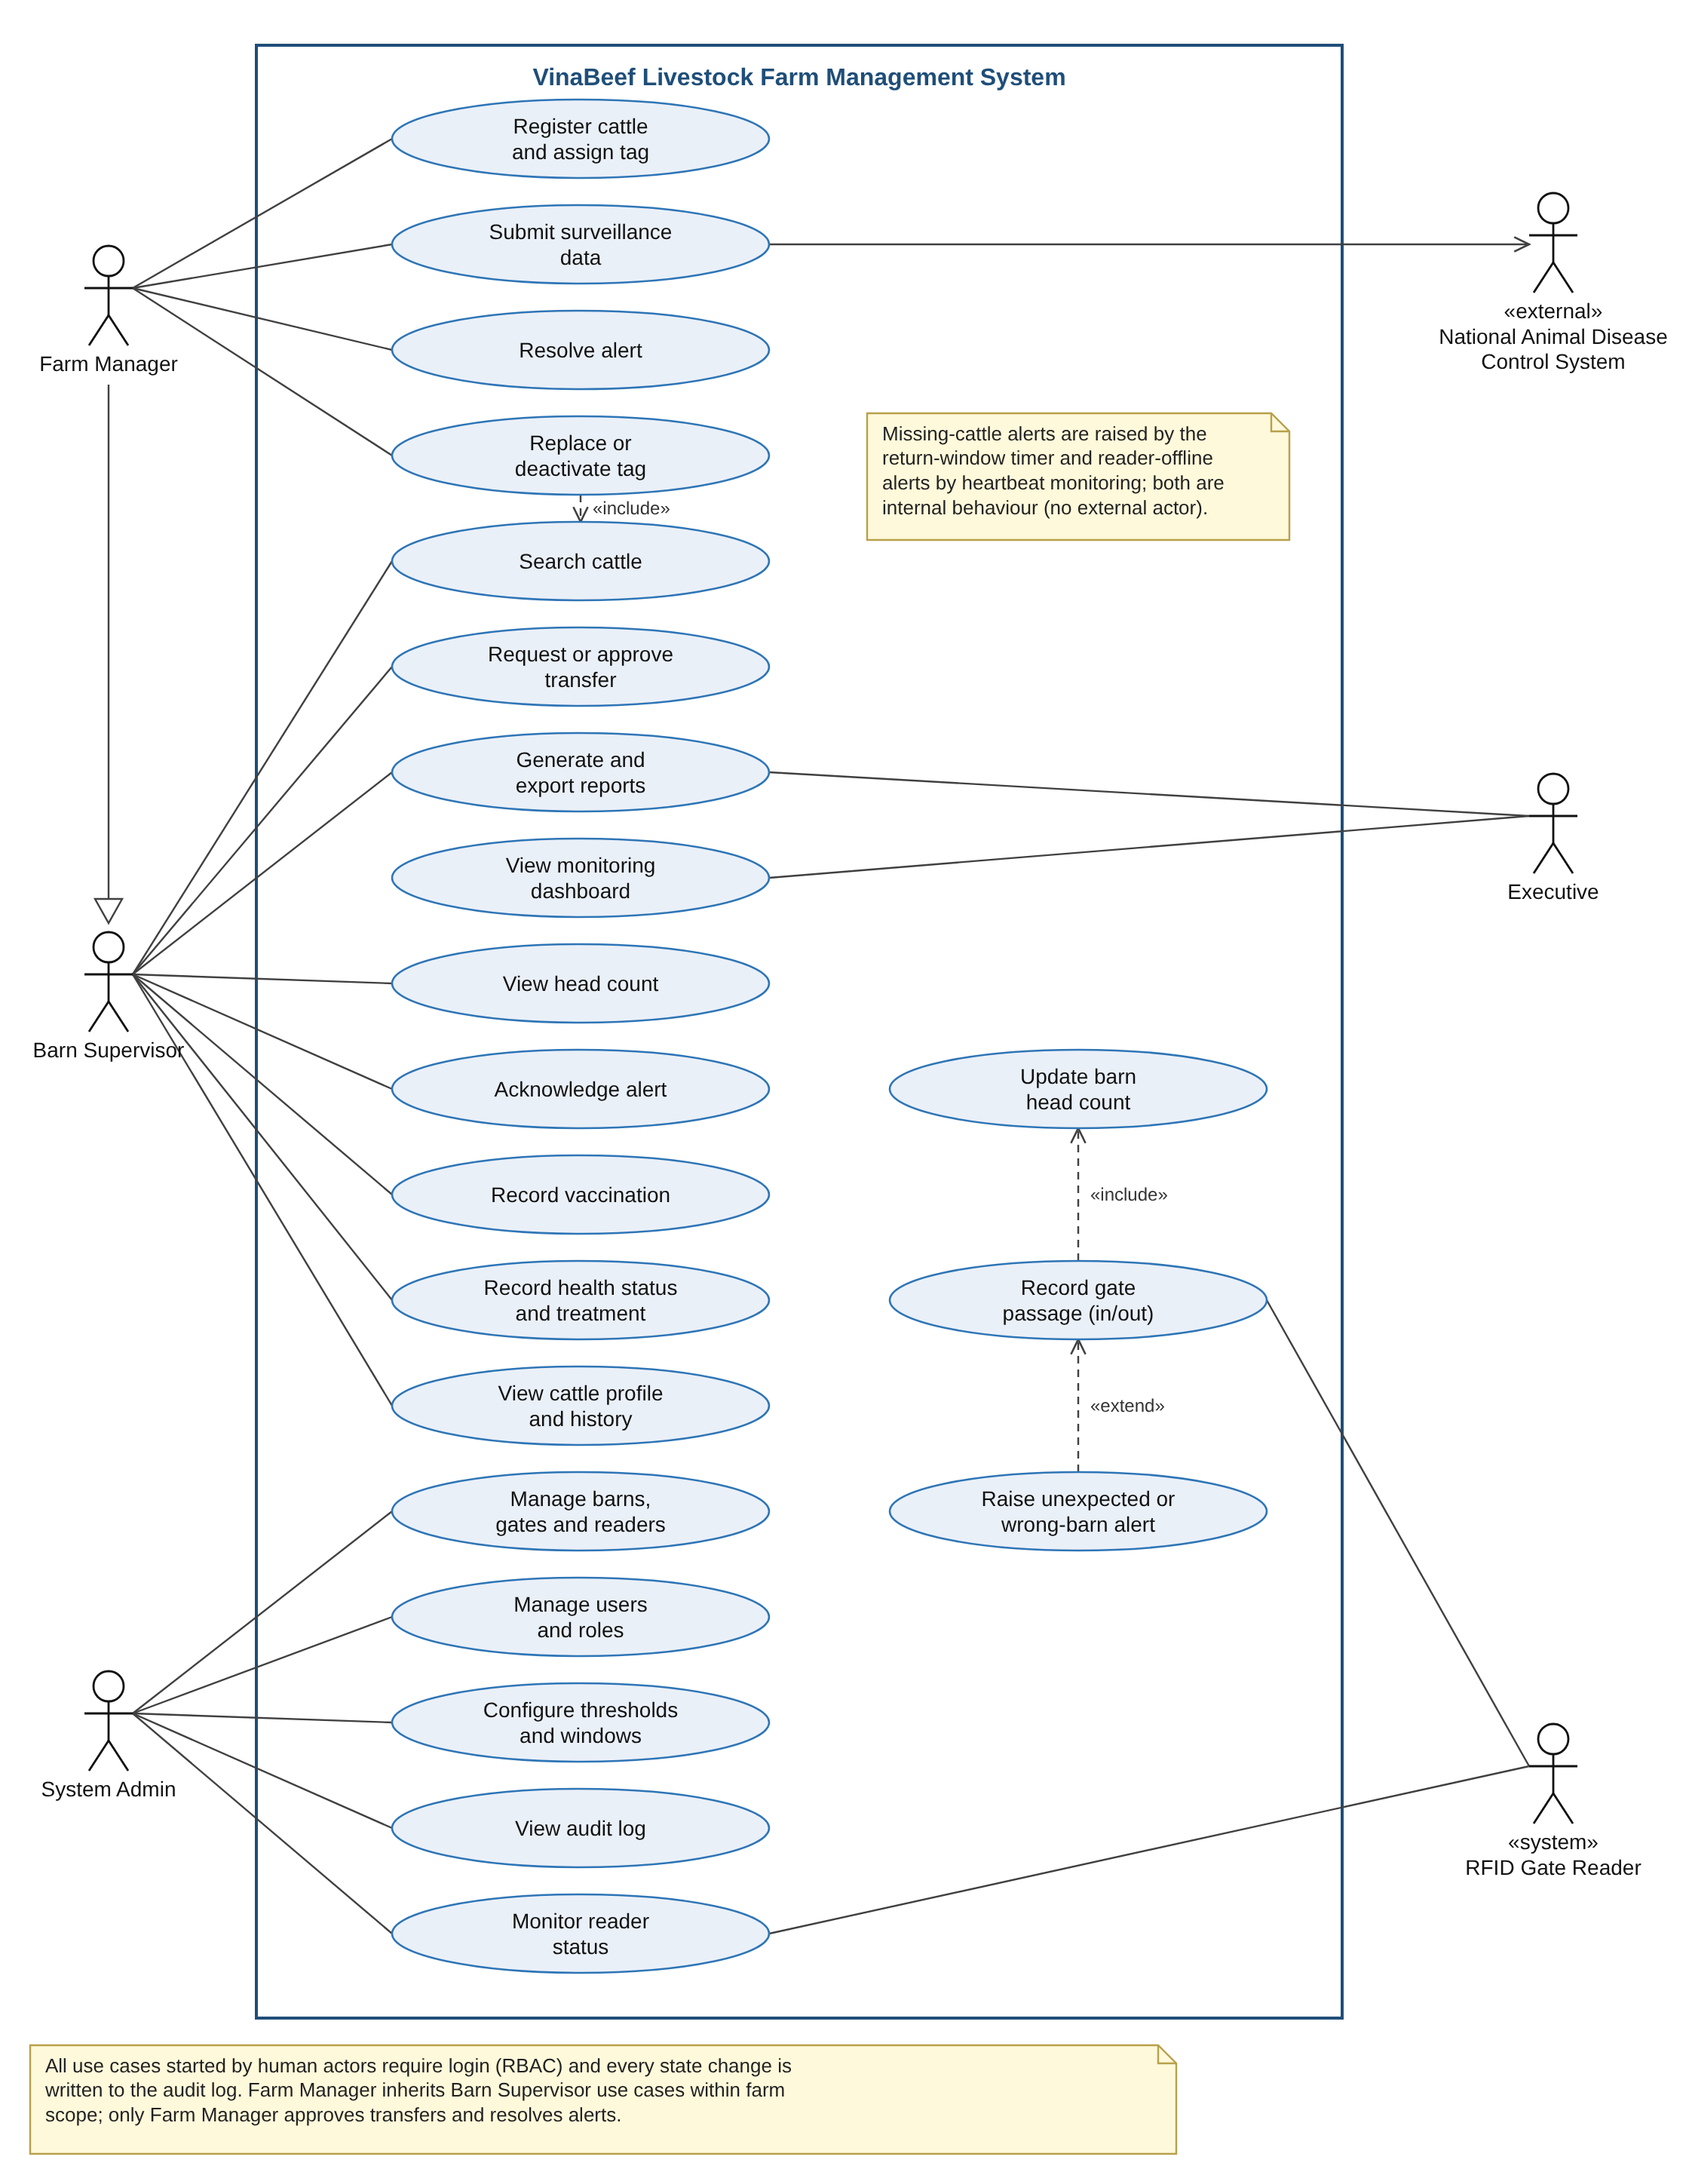
\includegraphics[width=\linewidth,height=0.8\textheight,keepaspectratio]{graphics/vinabeef/fig01-use-case-diagram.png}
\caption{Use case diagram}\label{fig:1}\end{figure}

\section{Requirements}\label{sec:2}

\subsection{Functional Requirements, Acceptance Criteria and Use Cases}\label{sec:2.1}

\subsubsection{Functional Requirements}\label{sec:2.1.1}

{\small
\begin{longtable}[]{|>{\raggedright\arraybackslash}p{\dimexpr 0.0967\linewidth-2\tabcolsep\relax}|>{\raggedright\arraybackslash}p{\dimexpr 0.1827\linewidth-2\tabcolsep\relax}|>{\raggedright\arraybackslash}p{\dimexpr 0.6906\linewidth-2\tabcolsep\relax}|}
\hline
\textbf{ID} & \textbf{Group} & \textbf{Requirement} \\ \hline
\endhead
\textbf{FR-01} & Cattle \& Tag & Register an animal with its RFID tag
and maintain its farm/barn assignment and animal profile \\ \hline
\textbf{FR-02} & Cattle \& Tag & Record lost/damaged physical-tag
incidents while preserving the permanent RFID identity and complete
history. A replacement tag carries the same permanent identity;
assigning a different RFID is outside the scope of this phase. \\ \hline
\textbf{FR-03} & Cattle \& Tag & Deactivate a tag when an animal dies or
leaves the company \\ \hline
\textbf{FR-04} & Cattle \& Tag & Search animals by tag, ID, farm or
barn \\ \hline
\textbf{FR-05} & Gate \& Reader & Manage farms, barns and gates \\ \hline
\textbf{FR-06} & Gate \& Reader & Register readers and map each to a
gate and direction \\ \hline
\textbf{FR-07} & Gate \& Reader & Monitor reader status through
heartbeats and alert when a reader is offline \\ \hline
\textbf{FR-08} & Movement & Capture read events automatically (tag,
reader, timestamp) \\ \hline
\textbf{FR-09} & Movement & Collapse repeated observations of the same
physical passage using reader/gate context and passage/direction state.
Retain distinct passages even within the time window; deduplicate
transport retries by stable event ID. \\ \hline
\textbf{FR-10} & Movement & Determine the direction of each passage
(IN/OUT) \\ \hline
\textbf{FR-11} & Movement & Maintain a near real-time head count per
barn \\ \hline
\textbf{FR-12} & Movement & Record observed movement and approved
barn/farm transfers separately. Change assigned custody only through a
versioned transfer workflow; cross-farm transfer requires source and
destination approvals. \\ \hline
\textbf{FR-13} & Alerting & Raise a missing-animal alert when animals
that left have not returned by the end of the return window \\ \hline
\textbf{FR-14} & Alerting & Raise an unexpected-animal alert for
unregistered or deactivated tags \\ \hline
\textbf{FR-15} & Alerting & Raise a wrong-barn alert when an animal
enters a barn it is not assigned to \\ \hline
\textbf{FR-16} & Health & Record vaccinations (such as: vaccine, batch,
date, veterinarian) and vaccination schedules \\ \hline
\textbf{FR-17} & Health & Record health status, diagnoses and
treatments \\ \hline
\textbf{FR-18} & Health & View an animal' s complete
profile and history timeline \\ \hline
\textbf{FR-19} & Reporting & Generate head count, movement, vaccination
coverage, health and alert reports \\ \hline
\textbf{FR-20} & Reporting & Export authorized reports in CSV,
PDF and XLSX formats, preserving the same selected records and scope
filters. \\ \hline
\textbf{FR-21} & Reporting & Send relevant outbreak and
health-surveillance data to the National Animal Disease Control System
via API. \\ \hline
\textbf{FR-22} & Reporting & Provide an executive monitoring dashboard
across farms \\ \hline
\textbf{FR-23} & Auditing & Maintain an audit log of relevant system
activities \\ \hline
\textbf{FR-24} & Administration & Manage users, roles and permissions \\ \hline
\textbf{FR-25} & Administration & Configure approved return windows,
reader-offline timing, alert notification settings and
passage-observation windows; configuration must not discard genuine
passages or hide missing cattle. \\ \hline
\end{longtable}
}

\subsubsection{Acceptance Criteria and Use Cases}\label{sec:2.1.2}

Acceptance criteria define observable functional outcomes. The following
representative fixtures verify the functional groups; timing, faults,
permissions and evidence completeness are additionally verified by the
QAS and SC tables. All implementation tests are planned for M2.

{\small
\begin{longtable}[]{|>{\raggedright\arraybackslash}p{\dimexpr 0.1633\linewidth-2\tabcolsep\relax}|>{\raggedright\arraybackslash}p{\dimexpr 0.8067\linewidth-2\tabcolsep\relax}|}
\hline
\textbf{Category} & \textbf{Acceptance Criteria} \\ \hline
\endhead
\textbf{Cattle \& Tag} & Register a previously unused permanent RFID
once; reject an active collision. Search returns the same cattle/history
after an identity-preserving physical-tag incident or deactivation. No
permanent RFID is reassigned to another animal. \\ \hline
\textbf{Gate \& Reader} & Provision an approved farm/barn/gate/reader
binding; reject inconsistent bindings. A heartbeat timeout records a
reader-offline alert under the declared timing policy; an available
reader resumes capture. \\ \hline
\textbf{Movement} & From declared initial occupancy, one valid OUT
followed by IN restores the count. Replayed event IDs have one effect.
OUT then IN within the observation window retains both passages.
Approved transfers retain source/destination history; an unexpected gate
read cannot silently change custody. \\ \hline
\textbf{Alerting} & An outstanding OUT at return-window close creates a
scoped missing alert; OUT/IN/OUT is outstanding again. An unregistered
tag or wrong-barn entry creates its respective alert. Approved custody
transfers are excluded from expected-return obligations; stale context
yields provisional alerts. \\ \hline
\textbf{Health} & One authorized vaccination/treatment intent and three
retries create one record. A schedule retains its due date/status and
links a completed dose without duplicate vaccination effects.
Corrections append linked versions; complete permitted history remains
retrievable. \\ \hline
\textbf{Reporting} & Export the same authorized dataset to CSV/PDF/XLSX
with identical record/scope selection. Executive views exclude clinical
narratives. Final external acceptance marks completion; 202 remains
pending; ambiguous outcomes preserve the approved intent. \\ \hline
\textbf{Auditing} & Every covered committed operation has valid source
evidence and eventually canonical evidence after collector recovery.
User and machine actors are identifiable; denied access never causes
unauthorized effects. \\ \hline
\textbf{Admin\-is\-tration} & Unapproved role/configuration changes and
self-escalation are denied. FM/EM approvals and SA application are
linked to scope and policy version; revoked access fails at report
execution/download. \\ \hline
\end{longtable}
}

\emph{\Cref{app:A} describes five core use cases, including approved
transfer and external-submission subflows. \Cref{fig:1} shows external
human, reader and National-system participation; timers and Edge Core
are internal behavior. Participation never grants unrestricted
permission.}

\subsection{Non-Functional Requirements}\label{sec:2.2}

VinaBeef must process gate reads within two seconds, preserve movement
and health records during normal operation, and enforce RBAC with
comprehensive audit logging. These constraints guide the
architecture alongside the current scale of three farms, 120 barns and
approximately 25,000 cattle. API exchange is an explicit function;
continuity, changeability and exchange quality require additional design
criteria.

E identifies an explicit assignment requirement, I a justified inference
and P a project-defined criterion. Timing boundaries, permissions and test
budgets marked P are set by this design because the assignment does not
specify them; they are verified in M2 and kept separate from the
assignment' s mandatory outcomes.

{\small
\begin{longtable}[]{|>{\raggedright\arraybackslash}p{\dimexpr 0.2426\linewidth-2\tabcolsep\relax}|>{\raggedright\arraybackslash}p{\dimexpr 0.2425\linewidth-2\tabcolsep\relax}|>{\raggedright\arraybackslash}p{\dimexpr 0.2425\linewidth-2\tabcolsep\relax}|>{\raggedright\arraybackslash}p{\dimexpr 0.2425\linewidth-2\tabcolsep\relax}|}
\hline
\textbf{ID} & \textbf{Characteristic} & \textbf{Required outcome and scope} & \textbf{Origin} \\ \hline
\endhead
NFR-01 & Performance & Each required gate read completes correctly
within \(\leq\)2 seconds under the declared peak workload & E
deadline; P completion boundary \\ \hline
NFR-02 & Reliability and durability & Zero lost movement or health
records during normal operation; correct effects and preserved history &
E no-loss; I/P recovery extension \\ \hline
NFR-03 & Availability and continuity & Local gate processing continues
during a 60-minute WAN outage; its backlog recovers within 10
minutes while live traffic continues & I continuity; P budgets \\ \hline
NFR-04 & Security & Enforce the four human roles with action and
barn/farm scope; deny unauthorized access and changes & E RBAC; P
detailed policy \\ \hline
NFR-05 & Auditability & Every covered committed operation has valid
durable evidence; sensitive access is also traceable & E comprehensive
audit; P coverage measure \\ \hline
NFR-06 & Interoperability & Exchange approved data through APIs with
durable submission state, validated formats and safe handling of
uncertain outcomes & E API function; I/P quality \\ \hline
NFR-07 & Scalability and configurability & Support the current dataset
and declared gate workload; compatible farm/barn/reader additions use
configuration and provisioning & E scale; I/P expansion \\ \hline
NFR-08 & Maintainability and testability & Compatible reader/API adapter
changes preserve core business rules and pass relevant contract/domain
tests & E SOLID/M2; I/P change criteria \\ \hline
\end{longtable}
}

\subsubsection{Performance and Record Preservation}\label{sec:2.2.1}

The assignment' s approximately 200 cattle per farm in 30
minutes gives 200/1800 = 0.111 passages/s. This average does not
establish instantaneous raw-read load: one passage can produce repeated
observations, and cattle can arrive in bursts. M2 workload declarations
must include read multiplicity, burst timing, concurrent farms and
available resources.

The measurement starts at read creation at the source and ends
at the correct durable local outcome: movement, count effect and
required evidence, or a valid duplicate/invalid-input disposition. A
queued message alone does not complete processing. Every required read
must meet the two-second limit; percentiles are diagnostic. Missing,
incorrect and timed-out outcomes remain in the result, with clock
uncertainty accounted for.

Each persistent owner commits its business effect, operation identity
and required evidence atomically, then reports success or acknowledges
delivery. Stable identities and idempotency prevent replay from
duplicating movements, vaccinations or treatments. Health retries after
an uncertain response resolve the original intent, and corrections
retain linked versions. Separately stored projections need their own
transaction and recovery boundaries; broker confirmation does not prove
application completion.

The no-loss requirement covers both movement and health. Process
restart/replay and WAN outage are design extensions covered while durable
storage remains intact and correctly configured. Lossless capture during
full-disk, power or storage destruction requires additional protection;
unrestricted disaster zero-loss is not assumed.

\subsubsection{Availability and External Exchange}\label{sec:2.2.2}

The offline subset includes gate capture, local movement/count,
alert evaluation with sufficient cached context, and durable pending
synchronization. Stale or unknown context is marked provisional.
Clinical operations, transfers, configuration changes and new human
login remain online-only. Existing local dashboard reads expire within 15 minutes of the last central policy validation, or earlier
session expiry; machine capture uses a separate provisioned identity and
policy.

At one logical movement per passage, a 60-minute test at 1/9 movement/s
creates 400 movements per farm, or 1,200 across three farms. Draining
this backlog in 600 seconds while accepting live traffic requires at
least 400/600 + 1/9 = 7/9 movement/s per farm at a movement-processing
stage. This is a necessary lower bound, not proof of end-to-end
capacity. The outage/recovery budgets are finite test budgets, not
production SLAs.

External submissions are persisted before dispatch. The integration
adapter distinguishes pending, unknown and completed outcomes. HTTP 202
is pending acceptance; a timeout can follow a receiver side effect.
Ambiguous operations are retried automatically only when the receiver
contract establishes safety; otherwise they require status lookup or
reconciliation. Backoff respects applicable Retry-After, and bounded
retries retain unresolved intents. The actual National API
contract must be qualified during implementation.

\subsubsection{Security and the RBAC Matrix}\label{sec:2.2.3}

Security is the characteristic; RBAC is an authorization mechanism.
Chapter 4 lists Authorization among cross-cutting concerns and defines
Security in terms of appropriate authorized access.
The matrix implements the assignment' s four
roles. Unspecified actions are denied, and permission is checked against
the canonical resource at the service, query and export boundaries.

BS = Barn Supervisor; FM = Farm Manager; SA = System Administrator; EM =
Executive Management. B/F means assigned barn/farm scope; H-B/H-F
permits complete history of cattle currently in that scope; O-F permits
own-origin records after a transfer; C is company technical scope; A is
an approved aggregate view; D means denied. Each permission also
requires the applicable approval, version and workflow checks.

{\footnotesize
\begin{longtable}[]{|>{\raggedright\arraybackslash}p{\dimexpr 0.1940\linewidth-2\tabcolsep\relax}|>{\raggedright\arraybackslash}p{\dimexpr 0.1940\linewidth-2\tabcolsep\relax}|>{\raggedright\arraybackslash}p{\dimexpr 0.1940\linewidth-2\tabcolsep\relax}|>{\raggedright\arraybackslash}p{\dimexpr 0.1940\linewidth-2\tabcolsep\relax}|>{\raggedright\arraybackslash}p{\dimexpr 0.1940\linewidth-2\tabcolsep\relax}|}
\hline
\textbf{Action group} & \textbf{BS} & \textbf{FM} & \textbf{SA} & \textbf{EM} \\ \hline
\endhead
Read gate count and alert dashboard & B & F & D & A \\ \hline
Read cattle identity and movement history & H-B & H-F or O-F & D & A \\ \hline
Read full vaccination and health profile & H-B & H-F or O-F & D & D \\ \hline
Register cattle and permanent RFID & D & F & D & D \\ \hline
Record vaccinations, treatments or schedules & H-B & H-F & D & D \\ \hline
Request health correction & H-B & H-F or O-F & D & D \\ \hline
Approve and apply health correction & D & O-F & D & D \\ \hline
Append metadata or movement correction & D & F or O-F & D & D \\ \hline
Request transfer & B & F & D & D \\ \hline
Approve barn or farm transfer & D & F & D & D \\ \hline
Acknowledge or request alert resolution & B & F & D & D \\ \hline
Resolve alert or approve domain configuration & D & F & D & D \\ \hline
Apply approved technical configuration & D & D & C & D \\ \hline
Generate and download business reports & B & F & D & A \\ \hline
Approve external submission or reconciliation & D & F & D & D \\ \hline
Read protected business audit evidence & B & O-F & D & A \\ \hline
Manage accounts and role grants & D & Approve F grants & Apply approved
C actions & Approve company SA/EM grants \\ \hline
Hard delete committed movement, health or audit & D & D & D & D \\ \hline
\end{longtable}
}

Cross-farm transfers require both source- and destination-scope
approvals. New health writes require current custody, a stable intent
and the expected version. Health correction approval belongs to the
original record' s farm; ordinary corrections cannot
change custody. FM approves business configuration before SA applies it.
Role grants require independent FM/EM approval and prohibit
self-escalation. SA has scoped technical/security audit access, without
ordinary clinical read/write privilege. Report execution and download
recheck current scope; aggregate permissions exclude clinical
narratives.

Provisioned readers and processing/synchronization/integration workers
have separate machine identities limited to their assigned duties; they
cannot impersonate human approvals. Compatible farm onboarding uses
preapproved deployment provisioning. Runtime farm-creation actions
require a separately defined approval policy and remain denied while
unmapped.

\subsubsection{Audit Coverage}\label{sec:2.2.4}

Auditability expresses the project' s traceability goal.
It is supported by Chapter 4' s Accountability and
Nonrepudiation concerns; logging contributes evidence
but does not alone establish strong nonrepudiation. The following
coverage groups operationalize comprehensive audit logging.

{\small
\begin{longtable}[]{|>{\raggedright\arraybackslash}p{\dimexpr 0.3234\linewidth-2\tabcolsep\relax}|>{\raggedright\arraybackslash}p{\dimexpr 0.3233\linewidth-2\tabcolsep\relax}|>{\raggedright\arraybackslash}p{\dimexpr 0.3233\linewidth-2\tabcolsep\relax}|}
\hline
\textbf{Covered event group} & \textbf{Evidence to retain} & \textbf{Responsible source} \\ \hline
\endhead
Cattle registration and device/configuration changes & Identity/scope,
validated versions, actor and approvals & Registry and
device/configuration owner \\ \hline
Movement, count, alert and transfer lifecycle & Read/operation
references, direction, effects, transition reasons and approvals &
Movement, Count and Alert owners \\ \hline
Vaccination, health, treatment and correction & Stable intent, protected
record/version links, reason and actor; clinical-access evidence &
Health owner \\ \hline
Authentication, authorization, accounts and grants & Decision,
role/resource scope, policy version, approver and applier & IAM and
resource owner \\ \hline
Reports, exports and audit access & Authorized scope, job/artifact,
execution/download/access result & Reporting and Audit owners \\ \hline
External submission and reconciliation & Intent, destination/schema,
attempt, status and acceptance evidence & Integration owner \\ \hline
Synchronization, evidence controls and restore & Source/receipt
identity, recovery/configuration reference and operator/result & Sync,
Audit and storage owners \\ \hline
\end{longtable}
}

Common fields identify who or which device/service acted, what action
affected which resource, when it occurred, its outcome and its
operation/correlation identity. Clinical text, secrets and credentials
are excluded from broad technical logs; protected references preserve
provenance.

Required business evidence/outbox commits with the mutation at its
source. Remote collection can recover later; failure to persist
mandatory source evidence prevents an audited business success. Relay
duplicates retain stable audit identities and are deduplicated.
Denied access remains denied if logging fails, and any missing required
evidence is an audit gap. Application roles cannot overwrite/delete
canonical facts; protection against unrestricted infrastructure
administrators requires separate controls.

\section{Architecture Characteristics}\label{sec:3}

\subsection{Identifying Candidate Architecture Characteristics}\label{sec:3.1}

Architecture characteristics express system success criteria.
The course requires a characteristic to concern quality beyond domain
functionality, influence design structure and matter to system success. Candidates were extracted from explicit requirements,
domain concerns and implicit knowledge. This
distinguishes qualities such as Security from tactics such as RBAC, and
Reliability from the choice of broker/database.

{\small
\begin{longtable}[]{|>{\raggedright\arraybackslash}p{\dimexpr 0.3234\linewidth-2\tabcolsep\relax}|>{\raggedright\arraybackslash}p{\dimexpr 0.3233\linewidth-2\tabcolsep\relax}|>{\raggedright\arraybackslash}p{\dimexpr 0.3233\linewidth-2\tabcolsep\relax}|}
\hline
\textbf{Candidate} & \textbf{Requirement origin} & \textbf{Structural influence} \\ \hline
\endhead
AC-01 Performance & E per-read deadline and workload & Completion
placement, queue scheduling and resource isolation \\ \hline
AC-02 Reliability/durability & E movement/health no-loss; P fault
extension & Persistence, commit/ACK boundaries, idempotency and
correction history \\ \hline
AC-03 Availability/continuity & I outage risk; P offline scope & Local
processing, cached context, pending storage and recovery \\ \hline
AC-04 Security & E RBAC; P scopes/guards & IAM, resource authorization
and human/machine identities \\ \hline
AC-05 Auditability & E comprehensive audit; P evidence policy & Source
evidence, collection, protection and traceable access \\ \hline
AC-06 Interoperability & E API exchange; I/P quality & Adapters, schema
validation and durable submission lifecycle \\ \hline
AC-07 Scalability/configurability & E current scale; I/P expansion &
Resource capacity, namespaces, configuration and provisioning \\ \hline
AC-08 Maintainability/testability & E SOLID and M2; I/P change criteria
& Stable core interfaces, replaceable adapters and deterministic
tests \\ \hline
\end{longtable}
}

Availability is a Reliability sub-characteristic in the course taxonomy. It has a separate criterion here so continuity is
measured independently of record preservation. Auditability elaborates
Accountability and is measured separately from permission correctness.
Semantic integrity and operational observability support these
candidates through correct identity/count interpretation and diagnosable
processing.

\subsection{Success Criteria}\label{sec:3.2}

Each criterion combines its characteristic, source, measurable outcome
and planned verification. The M1 criteria remain design contracts.
\Cref{sec:m2-health-results} records the subset exercised in the M2
Health backend.

{\small
\begin{longtable}[]{|>{\raggedright\arraybackslash}p{\dimexpr 0.2426\linewidth-2\tabcolsep\relax}|>{\raggedright\arraybackslash}p{\dimexpr 0.2425\linewidth-2\tabcolsep\relax}|>{\raggedright\arraybackslash}p{\dimexpr 0.2425\linewidth-2\tabcolsep\relax}|>{\raggedright\arraybackslash}p{\dimexpr 0.2425\linewidth-2\tabcolsep\relax}|}
\hline
\textbf{Criterion} & \textbf{Characteristic and source} & \textbf{Measurable acceptance} & \textbf{Planned verification} \\ \hline
\endhead
SC-01 & Performance; E/P, NFR-01 & Every required read completes
correctly within \(\leq\)2 seconds; zero missing outcomes or deadline
violations & Full input/outcome reconciliation and source/completion
timing, including uncertainty and failures \\ \hline
SC-02 & Reliability; E/P, NFR-02 & Zero missing committed
movement/health IDs or contents; no duplicate business effects within
the declared envelope & Input/history comparison; uncertain-response and
crash/replay controls \\ \hline
SC-03 & Availability; I/P, NFR-03 & Local gate core survives the
60-minute test; its backlog completes within 600 seconds of
recovery-ready while live traffic continues & Outage/live cohort IDs,
local timing, backlog and final central effects/evidence \\ \hline
SC-04 & Security; E/P, NFR-04 & All expected-deny cases reject without
protected disclosure or unauthorized effects; authorized controls
succeed & Role/action matrix plus wrong-scope, revocation, transfer and
export checks \\ \hline
SC-05 & Auditability; E/P, NFR-05 & Valid durable source evidence for
100\% of covered committed operations; required access events covered;
complete canonical set after recovery & Expected ID/content manifests;
source/collector faults and protected access controls \\ \hline
SC-06 & Interoperability; E/I/P, NFR-06 & Zero lost persisted intents;
valid approved payloads; no unsafe retries; completion requires
contractual acceptance evidence & API mocks for final success, 202, rate
limits and timeout-after-effect \\ \hline
SC-07 & Scalability; E/I/P, NFR-07 & Current dataset and declared
workload supported; compatible additions need zero core-rule edits and
preserve scopes/data & Dataset/load checks and preapproved
configuration-change demonstration \\ \hline
SC-08 & Maintainability; I/P, NFR-08 & Two compatible reader/API adapter
changes need zero core-rule edits; relevant contract/regression tests
pass & Frozen core-file diffs, interface review and repeatable domain
tests \\ \hline
\end{longtable}
}

Record reconciliation compares identities and contents, since matching
totals can hide a missing record and a duplicate. Availability recovery
is complete when the declared business/projection/evidence stages finish
the outage cohort; an empty queue alone is insufficient. External mock
results establish only the declared mock contract, not real National API
compatibility.

\subsection{Driving Characteristics}\label{sec:3.3}

The three driving characteristics are D-01 Reliability / Durability, D-02
Performance and D-03 Security / Auditability. Each combines a mandatory
outcome with independent structural consequences, and the course
recommends prioritization and keeping the primary list short. All three
are rated High importance and High difficulty: failing any of them
violates a mandatory requirement, and their interactions shape
persistence, timing and authorization. These ratings are design
assessments, not measured results.

\subsubsection{D01 Reliability and Durability}\label{sec:3.3.1}

Lost or duplicated movements corrupt counts, while lost health records
undermine complete profiles. This driver requires durable ownership,
atomic local effects/evidence, stable operation identities and preserved
correction history. It therefore affects stores, communication contracts
and recovery responsibilities. Additional writes, storage and
reconciliation are the trade-offs. Confirmation and ACK must match the
stage actually completed.

\subsubsection{D02 Performance}\label{sec:3.3.2}

The two-second deadline influences where gate processing completes and
which dependencies lie on its critical path. A low average passage rate
cannot rule out burst queues. Performance therefore remains a primary
driver even when average throughput seems modest.

The selected design completes the gate outcome locally and handles
central synchronization, reports and external delivery separately.
CPU/storage contention still requires resource control; local placement
alone proves no timing guarantee. The trade-off is balancing durable
work, concurrency and operating resources while retaining correctness
and audit. This requirement does not independently mandate
microservices.

\subsubsection{D03 Security and Auditability}\label{sec:3.3.3}

RBAC and comprehensive audit affect all protected operations. This
driver determines identity/resource boundaries, authorization placement,
workflow approvals and evidence ownership. Its costs include
authorization and durable-evidence work and restricted offline human
operations. Permission correctness and audit completeness remain
separate measures even though they share a driver group.

Availability remains significant for the selected edge/offline design,
with its own NFR, criterion and scenario. It is outside the primary
three because the assignment gives a mandatory timing constraint but no
outage duration or production availability target. Distributed styles
introduce latency, consistency and failure trade-offs, so \Cref{sec:4}
compares styles through concrete variants against these three drivers.

\subsection{Quality Attribute Scenarios}\label{sec:3.4}

Each scenario contains Source, Stimulus, Environment, Artifact, Response
and Response Measure, following the SEI formulation. QAS01--08 retain
the M1 scenarios. QAS09 and QAS10 extend them for on-site mobile
recording, where intermittent connectivity and cattle identification
errors can interrupt a clinical workflow.\cite{assignmentM2} Fixture
budgets are project-defined (P). \Cref{tab:m2-health-cases} records the
specific backend cases exercised in M2.

\subsubsection{QAS01 Correct and Timely Gate Processing}\label{sec:3.4.1}

{\small
\begin{longtable}[]{|>{\raggedright\arraybackslash}p{\dimexpr 0.4849\linewidth-2\tabcolsep\relax}|>{\raggedright\arraybackslash}p{\dimexpr 0.4851\linewidth-2\tabcolsep\relax}|}
\hline
\textbf{Element} & \textbf{Specification} \\ \hline
\endhead
Source & Qualified RFID reader or emulator with independently known
inputs, direction and source timing \\ \hline
Stimulus & Approximately 200 cattle pass one farm' s
gates in 30 minutes; declare raw-read multiplicity and burst schedule \\ \hline
Environment & Normal operation, healthy edge/storage, valid context and
current-scale dataset; resources declared \\ \hline
Artifact & Reader adapter and local movement/count/evidence
processing \\ \hline
Response & Commit each correct logical movement once; retain valid
duplicate/invalid-input dispositions and corresponding count effects \\ \hline
Response Measure & Every required read completes within \(\leq\)2
seconds from source creation, including clock uncertainty; zero
missing/incorrect outcomes or duplicate effects \\ \hline
\end{longtable}
}

Trace: NFR-01/02/05; SC-01/02/05; D-02 and D-01. Repeated observations
do not automatically represent additional cattle passages.

\subsubsection{QAS02 WAN Outage and Recovery}\label{sec:3.4.2}

{\small
\begin{longtable}[]{|>{\raggedright\arraybackslash}p{\dimexpr 0.4849\linewidth-2\tabcolsep\relax}|>{\raggedright\arraybackslash}p{\dimexpr 0.4851\linewidth-2\tabcolsep\relax}|}
\hline
\textbf{Element} & \textbf{Specification} \\ \hline
\endhead
Source & Network fault controller with provisioned reader/worker
identities \\ \hline
Stimulus & Disconnect central connectivity for 60 minutes; generate 400
valid movements/farm and restore services while live traffic
continues \\ \hline
Environment & Test with healthy local power/storage, sufficient
buffer and valid cached context \\ \hline
Artifact & Edge gate core/pending storage, Sync and central
business/count/evidence stages \\ \hline
Response & Continue local processing, identify stale context, retain
pending work and replay safely without blocking live gate processing \\ \hline
Response Measure & Preserve all 400 movements/farm without duplicate
effects; local reads retain SC-01; outage cohort finishes within 600
seconds of actual recovery-ready \\ \hline
\end{longtable}
}

Trace: NFR-03/01/02; SC-03/01/02; AC-03. Offline human operations follow
\Cref{sec:2.2.2}; three-farm testing uses 1,200 outage movements. The
budget applies to this finite cohort.

\subsubsection{QAS03 Consumer Crash and Replay}\label{sec:3.4.3}

{\small
\begin{longtable}[]{|>{\raggedright\arraybackslash}p{\dimexpr 0.4849\linewidth-2\tabcolsep\relax}|>{\raggedright\arraybackslash}p{\dimexpr 0.4851\linewidth-2\tabcolsep\relax}|}
\hline
\textbf{Element} & \textbf{Specification} \\ \hline
\endhead
Source & Fault controller and duplicate publisher \\ \hline
Stimulus & Crash after store commit but before ACK, restart and replay
the same 100 distinct normalized movement IDs \\ \hline
Environment & Intact storage; 100 distinct registered cattle initially
outside the barn; initial count zero; no new input. Repeat for
separately stored projections. \\ \hline
Artifact & Movement/count transactions, idempotency markers and required
source evidence \\ \hline
Response & Return the existing committed outcome; each store protects
its own marker/effect/evidence and acknowledges after commit \\ \hline
Response Measure & Exactly 100 IN movement/count effects and final count
100; zero missing/extra effects or required canonical facts within a
60 seconds of actual consumer recovery-ready \\ \hline
\end{longtable}
}

Trace: NFR-02/05; SC-02/05; D-01. Before-commit failure rolls back
together; same ID with different content is a conflict. The 60-second
budget is for this finite test cohort, not a production RTO or global
transaction guarantee.

\subsubsection{QAS04 Unauthorized Role or Scope}\label{sec:3.4.4}

{\small
\begin{longtable}[]{|>{\raggedright\arraybackslash}p{\dimexpr 0.4849\linewidth-2\tabcolsep\relax}|>{\raggedright\arraybackslash}p{\dimexpr 0.4851\linewidth-2\tabcolsep\relax}|}
\hline
\textbf{Element} & \textbf{Specification} \\ \hline
\endhead
Source & Authenticated BS/FM/SA/EM with a declared role and scope \\ \hline
Stimulus & Request protected data or mutation outside permission:
wrong-farm access, SA clinical write and revoked export. During WAN loss
also attempt online-only writes/new login and local dashboard reads
before and after lease expiry. \\ \hline
Environment & Online: authoritative policy and known allow/deny
fixtures. Offline: declared cached grant/scope and a known policy-lease
expiry; central revocation is observable only after reconnection or
lease expiry. \\ \hline
Artifact & Resource services, history queries, report execution/download
and audit source \\ \hline
Response & Enforce action/resource scope at the owner. Online checks use
current policy. Offline, only existing leased read-only dashboard access
and provisioned machine capture remain eligible; deny online-only
operations and expired leases. Retain required security evidence. \\ \hline
Response Measure & All declared allow/deny decisions are correct; denied
cases disclose no protected data and cause no unauthorized effect.
In-scope local reads succeed before the permitted expiry and are denied
at or after it. Online-only operations/new login fail during WAN loss;
audit gaps remain explicit. \\ \hline
\end{longtable}
}

Trace: NFR-04/05; SC-04/05; D-03; ADR-07/12. Test role/scope and
online/offline boundaries; gateway checks alone are insufficient.
Offline revocation exposure is bounded by the declared read-only lease,
rather than assumed instantaneous.

\subsubsection{QAS05 Health Write and Audit Failure}\label{sec:3.4.5}

{\small
\begin{longtable}[]{|>{\raggedright\arraybackslash}p{\dimexpr 0.4849\linewidth-2\tabcolsep\relax}|>{\raggedright\arraybackslash}p{\dimexpr 0.4851\linewidth-2\tabcolsep\relax}|}
\hline
\textbf{Element} & \textbf{Specification} \\ \hline
\endhead
Source & Authorized BS/FM and a fault controller \\ \hline
Stimulus & Submit one health intent and three same-payload retries while
either the remote collector is unavailable or required source evidence
insertion fails \\ \hline
Environment & Online health workflow; case A has healthy source storage,
case B fails the mandatory source evidence step \\ \hline
Artifact & Health version, operation receipt, source evidence/outbox and
collector \\ \hline
Response & A commits once with source evidence and relays later; B rolls
back and reports no success; resolve lost responses with the same
authorized intent \\ \hline
Response Measure & One intended health effect after a successful commit,
zero partial committed effects in B before repair; complete history and
source evidence; the small canonical audit cohort completes within a
30 seconds of collector-ready \\ \hline
\end{longtable}
}

Trace: NFR-02/05/04; SC-02/05/04; D-01/D-03. Reauthorization and
matching prior receipts prevent a retry from becoming a second
treatment. The 30-second budget applies to this finite cohort, not a
global audit-delivery SLA.

\subsubsection{QAS06 Ambiguous External Delivery}\label{sec:3.4.6}

{\small
\begin{longtable}[]{|>{\raggedright\arraybackslash}p{\dimexpr 0.4849\linewidth-2\tabcolsep\relax}|>{\raggedright\arraybackslash}p{\dimexpr 0.4851\linewidth-2\tabcolsep\relax}|}
\hline
\textbf{Element} & \textbf{Specification} \\ \hline
\endhead
Source & External API mock and network fault controller \\ \hline
Stimulus & Return 202, rate limits or timeout after a receiver side
effect; provide separate contracts with and without idempotency \\ \hline
Environment & Persisted approved intent/schema; receiver safety
semantics explicitly declared; gate processing independent \\ \hline
Artifact & Integration adapter, durable intent/attempt states and
reconciliation path \\ \hline
Response & Retain pending/unknown outcomes; respect applicable
Retry-After and bounded retries; retry ambiguous operations only when
contractually safe \\ \hline
Response Measure & Zero lost intents; one receiver effect in the
idempotent fixture; no blind ambiguous retry without safety; Delivered
only after final business acceptance evidence \\ \hline
\end{longtable}
}

Trace: NFR-06/02; SC-06/02; AC-06. Retry-budget exhaustion retains
unresolved work. Mocks cannot establish actual National API
capabilities.

\subsubsection{QAS07 Compatible Configuration Growth}\label{sec:3.4.7}

{\small
\begin{longtable}[]{|>{\raggedright\arraybackslash}p{\dimexpr 0.4849\linewidth-2\tabcolsep\relax}|>{\raggedright\arraybackslash}p{\dimexpr 0.4851\linewidth-2\tabcolsep\relax}|}
\hline
\textbf{Element} & \textbf{Specification} \\ \hline
\endhead
Source & Deployment team using a preapproved farm/barn/reader
provisioning package \\ \hline
Stimulus & Add a compatible farm namespace and reader bindings through
configuration \\ \hline
Environment & Current three-farm dataset; synthetic additional farm,
approved identities/scopes and allocated resources \\ \hline
Artifact & Registry/configuration, routing, scope policy and core
business modules \\ \hline
Response & Validate/provision bindings, preserve existing records and
isolate the new scope \\ \hline
Response Measure & Zero edits to predeclared core movement/count/health
rules; correct positive/negative scope checks; existing workload retains
SC-01 before and after change \\ \hline
\end{longtable}
}

Trace: NFR-07/01/04; SC-07/01/04; AC-07. This verifies compatible
onboarding, not unlimited capacity or an undefined runtime creation
permission.

\subsubsection{QAS08 Compatible Adapter Changes}\label{sec:3.4.8}

{\small
\begin{longtable}[]{|>{\raggedright\arraybackslash}p{\dimexpr 0.4849\linewidth-2\tabcolsep\relax}|>{\raggedright\arraybackslash}p{\dimexpr 0.4851\linewidth-2\tabcolsep\relax}|}
\hline
\textbf{Element} & \textbf{Specification} \\ \hline
\endhead
Source & Developer in development/CI \\ \hline
Stimulus & Independently replace a reader protocol adapter and an API
adapter while preserving their domain-facing contracts \\ \hline
Environment & M2 implementation, frozen core-file inventory and
deterministic domain/contract fixtures \\ \hline
Artifact & Adapter interfaces/configuration and core
movement/count/health modules \\ \hline
Response & Implement changes at the adapter boundary and run relevant
contract/domain/regression tests \\ \hline
Response Measure & Both compatible changes require zero core-rule edits;
relevant tests pass and repeated deterministic fixtures yield expected
outcomes \\ \hline
\end{longtable}
}

Trace: NFR-08; SC-08; AC-08 and SOLID. Domain-semantic changes need
separate analysis; absent implementation produces Not Run.

\newpage
\subsubsection{QAS09 Mobile Capture and Restart}\label{sec:qas09}

{\small
\begin{longtable}{|p{0.19\linewidth}|p{0.72\linewidth}|}
\hline
\textbf{Element} & \textbf{Specification} \\ \hline
\endhead
Source & An authorized barn supervisor uses a mobile client and
reader. A tester interrupts connectivity or restarts the app. \\ \hline
Stimulus & Scan and confirm the animal, enter the clinical details, and
attempt to save. Interrupt connectivity before or after saving, then
reconnect and retry with the same intent ID. \\ \hline
Environment & The tag and custody start in the verified scope. The
client loses and regains network access. Option A follows the online-only
baseline. Option B proposes durable local drafts during the outage. \\ \hline
Artifact & Mobile form, local draft store and sync state, together with
the Health intent, receipt, clinical record and source evidence. \\ \hline
Response & Under A, the app reports that a new offline save is unavailable.
Under B, the app reports a saved draft only after the local commit and
restores the same cattle, actor, intent and content after restart. Upon
reconnection, Health checks current authorization, custody and version.
The app shows acceptance only after the server confirms the result. \\ \hline
Response\newline Measure & Zero server acceptances during the outage and zero
false saved or accepted states. For B, the proposed fixture restores
20 of 20 acknowledged drafts. With unchanged rights and reconnection
ready, the valid cohort yields 20 matching effects, receipts and evidence
rows within 120 seconds (P), with zero duplicates or wrong-cattle effects.
Conflicts retain their actual nonaccepted outcome. \\ \hline
\end{longtable}
}

Trace: SC-02 and SC-05, \Cref{adr:12}, and T05/T06. Offline drafts and
their proposed measures remain design-only pending confirmation of
scope. The online retry controls are recorded in
\Cref{tab:m2-health-cases}.

\newpage
\subsubsection{QAS10 Cattle Identity and Current Authorization}\label{sec:qas10}

{\small
\begin{longtable}{|p{0.19\linewidth}|p{0.72\linewidth}|}
\hline
\textbf{Element} & \textbf{Specification} \\ \hline
\endhead
Source & A barn supervisor or farm manager, an out-of-scope user,
the RFID reader and an administrator who can change grants or custody. \\ \hline
Stimulus & Scan an unknown, deactivated or ambiguous tag. Attempt a
submission, retry, or receipt or history read after a grant or custody
change, or submit with a stale resource version. \\ \hline
Environment & Health is online with server-owned cattle and custody data.
Allow and deny cases declare the caller's current grants, resource
version and expected cattle binding. \\ \hline
Artifact & Scan and form selection, verified principal and grants,
canonical cattle and record context, Health policy and clinical outcome. \\ \hline
Response & Require explicit cattle confirmation before capture. An unknown
tag stays unresolved. A known deactivated tag still resolves to cattle
identity and history for authorized callers, and cannot start a new
clinical write. Each protected operation checks current rights. A
new submission with a stale version goes to review when scope still
allows it. A committed retry follows current receipt authorization.
An out-of-scope lookup gives no cattle data. \\ \hline
Response\newline Measure & Zero unauthorized effects or protected-data
disclosures in deny cases. Unknown tags create zero cattle records.
For allowed flows, the confirmed cattle and submitted content match
the resulting receipt and history. A stale uncommitted intent produces
zero clinical records, and an authorized replay produces no extra
effect. \\ \hline
\end{longtable}
}

Trace: SC-02, SC-04 and SC-05, \Cref{adr:07,adr:08}, and T06--T09.
\Cref{tab:m2-health-cases} covers the backend examples exercised on
\texttt{staging}. The mobile confirmation flow and integration with
the real identity and grant providers remain pending.

\section{Architecture Structure}\label{sec:4}

\subsection{Candidate Architecture Styles}\label{sec:4.1}

Six architecture families are evaluated as concrete VinaBeef variants,
using the course trade-off framework and supplemental style
descriptions. The comparison also includes V2E, a modular
central monolith with the same farm edge as V4, so placement benefits
are not mistaken for benefits unique to service-based architecture. D-01
Reliability/Durability, D-02 Performance and D-03 Security/Auditability
are primary; Availability is secondary.


\begin{itemize}
  \item \textbf{V1 Layered monolith:} one central deployable unit with presentation, business and persistence layers. Readers send every read across the WAN to the central site. A single ACID database makes it easy to commit a business effect and its evidence atomically (D-01, D-03). However, every read' s deadline then depends on WAN latency (D-02), and gate processing stops during an outage.
  \item \textbf{V2 Modular monolith:} the same deployment as V1, split internally into domain modules (Movement, Health, Registry, Alerting). Module boundaries are clearer than in V1, but it has the same timing and continuity limits.
  \item \textbf{V3 Microkernel:} a core system with plug-ins for reader protocols, report exporters and API adapters. This suits adapter variation (NFR-08) but does not structure the whole system, and plug-ins widen the trust boundary.
  \item \textbf{V4 Service-based with farm edge:} a few coarse-grained domain services, each owning its own schema, plus an edge gateway at each farm that completes gate processing locally.
  \item \textbf{V5 Event-driven (broker topology):} every processing step reacts to events through a central broker. This buffers bursts and decouples producers from consumers. However, each hop adds latency, and a broker acknowledgement does not prove that the business outcome is complete. Authorization and audit context are also harder to trace across asynchronous chains.
  \item V2E Modular monolith with farm edge: the same qualified local core, commit boundary and offline subset as V4, but one modular central deployable application. Local deadline and outage support are comparable; central deployment and process-resource isolation differ.
  \item V6 Microservices with the same farm edge: each farm runs the same local core, atomic commit boundary and offline subset as V4. Only the central backend is decomposed into finer-grained services with separately owned databases. WAN and central broker hops are outside the local gate deadline. Cross-owner workflows may need durable coordination; the added authorization, evidence and deployment boundaries require qualification.
\end{itemize}


\subsection{Comparison}\label{sec:4.2}

Each variant is rated from 1 (poor fit) to 5 (excellent fit) for this
project. The three drivers have weight 3, Availability has weight 2, and
Simplicity/Cost and Evolvability have weight 1 each; the maximum is 65.
Ratings are the group's assessments of the stated design and control effort,
not measured guarantees or inherent limits of a style. V4, V2E and V6
share the same local gate core, so their local Performance and
normal-operation Reliability/Durability ratings are equal. V6 scores
47/65; its additional central policy/evidence boundaries and deployment
cost drive the remaining differences.

{\footnotesize
\begin{longtable}[]{|>{\raggedright\arraybackslash}p{\dimexpr 0.1678\linewidth-2\tabcolsep\relax}|>{\raggedright\arraybackslash}p{\dimexpr 0.1162\linewidth-2\tabcolsep\relax}|>{\raggedright\arraybackslash}p{\dimexpr 0.1340\linewidth-2\tabcolsep\relax}|>{\raggedright\arraybackslash}p{\dimexpr 0.1243\linewidth-2\tabcolsep\relax}|>{\raggedright\arraybackslash}p{\dimexpr 0.1211\linewidth-2\tabcolsep\relax}|>{\raggedright\arraybackslash}p{\dimexpr 0.1114\linewidth-2\tabcolsep\relax}|>{\raggedright\arraybackslash}p{\dimexpr 0.1226\linewidth-2\tabcolsep\relax}|>{\raggedright\arraybackslash}p{\dimexpr 0.0727\linewidth-2\tabcolsep\relax}|}
\hline
\textbf{Variant} & \textbf{D-01 Reliability / Durability (\(\times\)3)} & \textbf{D-02 Performance (\(\times\)3)} & \textbf{D-03 Security / Auditability (\(\times\)3)} & \textbf{Avail\-abil\-ity (\(\times\)2)} & \textbf{Sim\-plic\-ity / Cost (\(\times\)1)} & \textbf{Evolv\-abil\-ity (\(\times\)1)} & \textbf{Total} \\ \hline
\endhead
\textbf{V1 Layered monolith} & 3 & 2 & 4 & 1 & 5 & 1 & 35 \\ \hline
\textbf{V2 Modular monolith} & 3 & 2 & 4 & 1 & 4 & 2 & 35 \\ \hline
\textbf{V3 Microkernel} & 3 & 2 & 3 & 1 & 4 & 3 & 33 \\ \hline
\textbf{V4 Service-based + farm edge} & \textbf{4} & \textbf{4} &
\textbf{4} & \textbf{4} & \textbf{3} & \textbf{3} & \textbf{50} \\ \hline
\textbf{V5 Event-driven} & 4 & 3 & 2 & 3 & 2 & 4 & 39 \\ \hline
V6 Microservices + same farm edge & 4 & 4 & 3 & 4 & 1 & 5 & 47 \\ \hline
V2E Modular monolith + same farm edge & 4 & 4 & 4 & 4 & 4 & 2 & 50 \\ \hline
\end{longtable}
}

\textbf{Rationale per driver}


\begin{itemize}
  \item \textbf{D-01 Reliability/Durability:}
  \begin{itemize}
    \item The explicitly central-only variants V1--V3 score 3 under this comparison. A single database supports atomic commits, but source capture and WAN receipt still require qualified protection. This is not an inherent prohibition on adding an edge to a monolith.
    \item V4 commits each read at the edge together with its operation identity and evidence before acknowledging it. It then relays the read through an outbox to central.
    \item V5 has a durable broker and replay, but scores only 4 because the broker acknowledgement must not be mistaken for business completion.
    \item V2E and V6 use the same farm-local commit contract as V4 and receive the same Reliability/Durability rating of 4. V6 must preserve receipts, source evidence and owned recovery for central workflows; separate databases do not inherently lose records. Cross-owner workflows require explicit coordination where atomicity cannot be kept within one owner.
  \end{itemize}
  \item \textbf{D-02 Performance:} the \(\leq\)2 second deadline applies to every read, so what matters is where processing completes and how many hops lie on the critical path, not average throughput.
  \begin{itemize}
    \item V4, V2E and the stated V6 all complete the same gate outcome on the farm LAN and receive Performance 4. Their central decomposition does not add a WAN or central broker hop to this local completion path.
    \item In V1--V3, every read depends on the WAN.
    \item The stated V5 broker topology puts central broker/network hops on the gate path. V6 does not: only its central backend is split into microservices. Resource contention and actual timing must still be measured in M2 for every variant.
  \end{itemize}
  \item \textbf{D-03 Security/Auditability:}
  \begin{itemize}
    \item V1, V2, V2E and V4 have few authorization boundaries and can commit source evidence in the same transaction as the business change.
    \item V5 carries authorization/evidence context across asynchronous chains. V6 receives Security/Auditability 3 because its finer central boundaries add policy propagation, evidence correlation and review effort. It can satisfy the same mandatory controls; this rating assesses project fit, not permission correctness or audit loss already observed in an implementation.
  \end{itemize}
  \item Availability (secondary): V4, V2E and the stated V6 have the same farm-local core, offline subset and Availability rating of 4. Central service granularity does not determine whether this gate subset survives WAN loss.
\end{itemize}


\subsection{Selected Style}\label{sec:4.3}

\textbf{Decision: V4 is selected. V4 and V2E both score 50/65, and V6
with the same farm edge scores 47/65; all three can implement the same
local gate contracts. V4 is chosen for explicit ownership and separate
process/deployment boundaries between movement, clinical work,
reporting/integration and identity/admin, with fewer central service
units than V6. V2E remains a credible alternative with simpler central
deployment. The shared central PostgreSQL server remains a common fault
domain, mitigated by the synchronous standby and backups in
\Cref{sec:4.5}.}


\begin{itemize}
  \item \textbf{D-01 Reliability/Durability:}
  \begin{itemize}
    \item The edge commits the movement, count effect, operation identity and source evidence in one local transaction before it acknowledges the read.
    \item A transactional outbox relays the committed facts to central at least once. Stable identities make replays idempotent.
  \end{itemize}
  \item \textbf{D-02 Performance:}
  \begin{itemize}
    \item The critical path from read to durable local outcome stays inside one farm, with no WAN, central broker or external API on it.
    \item Central synchronization, reporting and National API delivery run outside the deadline path.
    \item Resource isolation on the edge is still required. Local placement makes the deadline achievable but does not guarantee it.
  \end{itemize}
  \item \textbf{D-03 Security/Auditability:}
  \begin{itemize}
    \item A small number of coarse-grained services keeps authorization and evidence ownership clear. Each service authorizes against its own resources and commits its audit evidence in the same transaction as the change.
    \item The API gateway authenticates users and applies coarse checks. Services re-check permissions on the canonical resource, because gateway checks alone are insufficient.
  \end{itemize}
  \item \textbf{Role of event-driven:} events propagate facts that are already committed: edge to central, movement to head count and alerts, and health records to integration. This keeps the benefits of buffering and decoupling without putting broker hops on the deadline path.
  \item \textbf{Availability (secondary):} the same edge placement lets gate processing continue during a WAN outage.
  \item \textbf{Rejected -- central-only V1/V2:} their gate outcomes depend on the WAN. This does not reject modular monolith + edge (V2E), which remains a viable alternative; V4 is preferred for central domain ownership and isolation.
  \item \textbf{Rejected -- V5 pure event-driven:} broker hops on the critical path, and audit context is harder to trace end to end. Event-driven is kept only as a communication pattern inside V4.
  \item \textbf{Not selected -- V6 microservices with the same farm edge:} it can meet the same local deadline and preservation contracts, but its additional central deployment, policy and evidence coordination is not justified without a need for finer independent scaling or releases. This reflects project fit and operating cost, not an inherent weakness of microservices in reliability or security.
  \item \textbf{Accepted trade-offs:} edge software must be deployed and operated at three sites, and central views are eventually consistent with the farms.
\end{itemize}


\subsection{Logical Architecture}\label{sec:4.4}

\subsubsection{Step 1: Identify components from workflows and quality constraints}

The core workflows produce Cattle Registry, Device Management, Movement
Processing, Head Count, Alerting, Health Records, Reporting and
Integration Gateway. Identity \& Access and Audit support protected
operations. Farm Edge Core is the deployment name for the Edge Gateway
in the NFR and traceability tables; it executes local
movement/count/provisional-alert logic, while central components
consolidate the same committed facts. A logical component is not
automatically a separately deployed service.

\subsubsection{Step 2: Assign functional and quality requirements}

{\small
\begin{longtable}[]{|>{\raggedright\arraybackslash}p{\dimexpr 0.3233\linewidth-2\tabcolsep\relax}|>{\raggedright\arraybackslash}p{\dimexpr 0.3233\linewidth-2\tabcolsep\relax}|>{\raggedright\arraybackslash}p{\dimexpr 0.3233\linewidth-2\tabcolsep\relax}|}
\hline
\textbf{Component} & \textbf{FR coverage} & \textbf{Quality responsibilities} \\ \hline
\endhead
Cattle Registry & FR-01..04, shared FR-12/18 & Permanent identity,
custody version, RBAC and source evidence \\ \hline
Device Management & FR-05..07 & Approved reader bindings, heartbeat and
versioned farm context \\ \hline
Movement Processing / farm local core & FR-08..10, shared FR-12 &
Passage identity/direction, durable receipt/fact/evidence;
NFR-01/02/03 \\ \hline
Head Count & FR-11 & Declared initial state, idempotent effects and
rebuildable scoped projections \\ \hline
Alerting & FR-13..15,25 & Unmatched-return obligations,
wrong-barn/unexpected rules; scoped lifecycle \\ \hline
Health Records & FR-16..18 & Stable intent, vaccination schedules,
append-only corrections and complete permitted history \\ \hline
Reporting & FR-19,20,22 & CSV/PDF/XLSX, aggregate views and scope
rechecks at execution/download \\ \hline
Integration Gateway & FR-21 & Durable approved intent;
contract-qualified retries and final evidence \\ \hline
Identity \& Access & FR-24 & NFR-04 Security; human/machine identity,
role grant and resource policy \\ \hline
Audit & FR-23 & NFR-05 Auditability; source evidence, protected
collection and access \\ \hline
Edge Core / sync & FR-08..11,13..15, shared FR-07/25 & Local two-second
outcome, provisional context and recoverable relay \\ \hline
\end{longtable}
}

\subsubsection{Step 3: Refine responsibilities and ownership}

Reader observations are classified into passages using qualified
gate/antenna context and direction state. A time window collapses
observations of the same passage; it cannot suppress a genuine return
passage. Transport replay is separately deduplicated by stable IDs. Head
Count starts from an approved occupancy snapshot and applies each
accepted effect once; inconsistent or unresolved reads retain a durable
disposition and make uncertainty explicit.

Observed location and assigned custody are separate. A gate read updates
movement history and observed occupancy, but cannot authorize a
transfer. Cross-farm custody changes require both farm approvals and the
expected custody version. Missing detection tracks outstanding OUT
passages matched only by a later valid IN, excluding approved custody
transfers; OUT/IN/OUT creates a new outstanding obligation.

Identity \& Access provides authentication, grants and a shared policy
library. Every resource owner enforces action/scope on canonical
resources. Each business owner commits its required evidence locally;
Audit collection is asynchronous and recoverable. Separation into
logical modules does not imply a remote call between them.

\subsubsection{Step 4: Check the characteristics}

Performance: source creation to the correct durable local outcome is the
completion boundary defined in
\Cref{sec:2.2.1}. That path has no WAN or central dependency
and is measured for every required read; actual timing remains Planned
for M2. Reliability: each owner commits effect, operation receipt and
required source evidence atomically before success/ACK; projections have
their own idempotent transactions. Availability: local gate core and
versioned cached context support the declared offline subset; stale
alerts are provisional. Security/Auditability: canonical action/scope
checks, approval guards and source evidence apply throughout.
Interoperability uses an isolated, contract-qualified adapter. Growth
and adapter changes follow SC-07/08.

\subsubsection{Step 5: Final interactions and architectural views}

{\small
\begin{longtable}[]{|>{\raggedright\arraybackslash}p{\dimexpr 0.3233\linewidth-2\tabcolsep\relax}|>{\raggedright\arraybackslash}p{\dimexpr 0.3233\linewidth-2\tabcolsep\relax}|>{\raggedright\arraybackslash}p{\dimexpr 0.3233\linewidth-2\tabcolsep\relax}|}
\hline
\textbf{From / to} & \textbf{Contract} & \textbf{Timing boundary} \\ \hline
\endhead
Reader $\rightarrow$ farm Edge Core & Qualified read observation;
classification and durable disposition & Source-to-local-outcome
\(\leq\)2 s; NFR-01 \\ \hline
Local modules $\rightarrow$ edge store & Atomic
fact/count/receipt/source evidence/outbox & Commit before gate
success \\ \hline
Edge outbox $\rightarrow$ broker $\rightarrow$ central owner &
At-least-once stable facts; publisher confirm distinct from consumer ACK
& Outside gate deadline \\ \hline
Central owner $\rightarrow$ projection workers & Durable outbox work;
atomic projection marker/effect/evidence & Restart/replay safe; included
in recovery completion \\ \hline
Registry/devices $\rightarrow$ edge caches & Versioned assignments and
approved configuration & Refresh outside local gate critical path \\ \hline
Clients $\rightarrow$ gateway $\rightarrow$ resource owner &
Authentication plus action/scope/approval checks & Online except
authorized leased local reads \\ \hline
Business evidence $\rightarrow$ Audit & Protected source outbox,
stable audit ID and recoverable collection & Source commit mandatory;
collection can recover later \\ \hline
Reporting $\rightarrow$ service API/event read model & Owned data
contracts, no cross-schema reads & Freshness shown; current scope
rechecked \\ \hline
Integration $\rightarrow$ National API & Persisted approved intent,
qualified retry/status contract & No gate dependency; final contractual
acceptance only \\ \hline
\end{longtable}
}

\begin{figure}[htbp]\centering
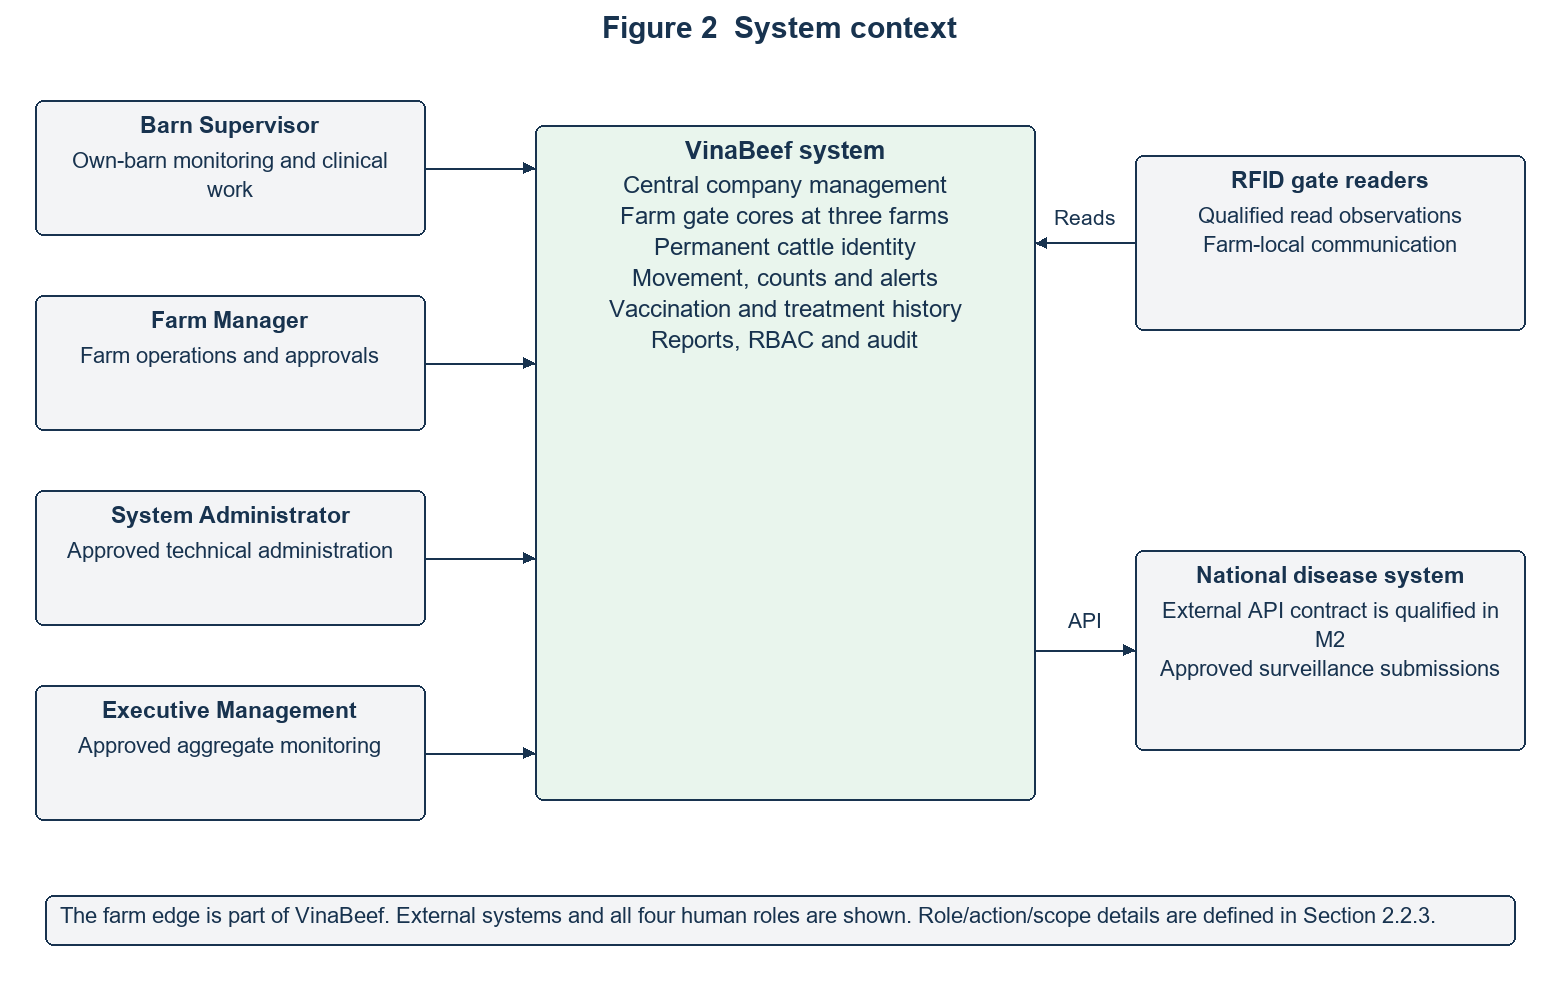
\includegraphics[width=\linewidth,height=0.42\textheight,keepaspectratio]{graphics/vinabeef/fig02-system-context.png}
\caption{System context with all four human roles}\label{fig:2}\end{figure}

\begin{figure}[htbp]\centering
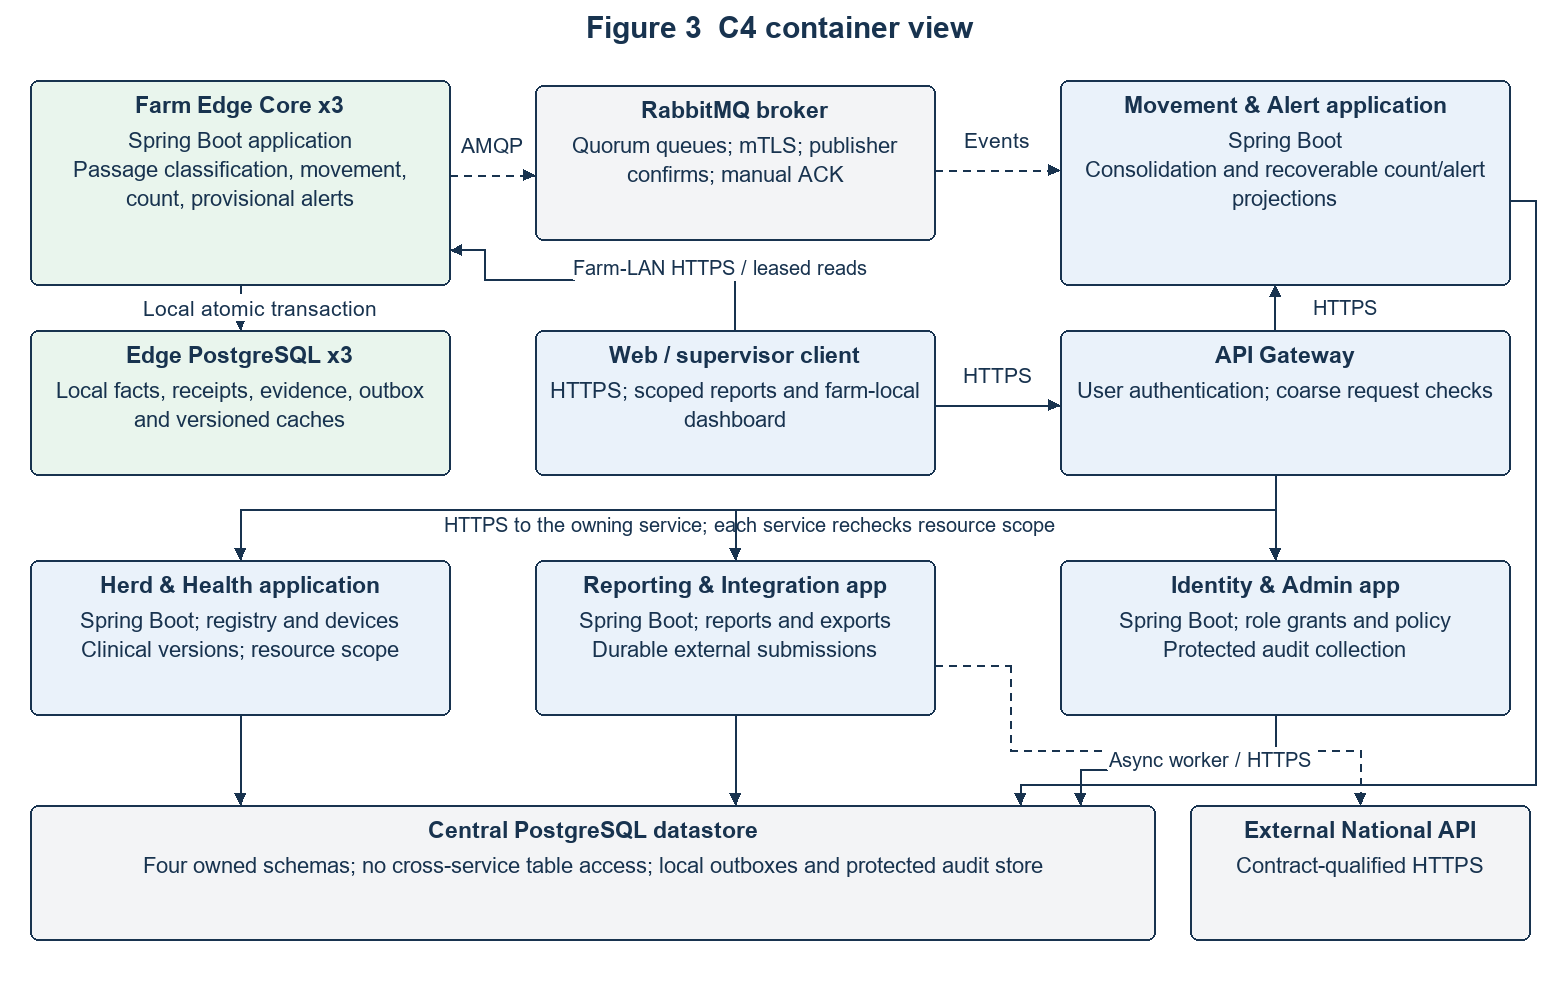
\includegraphics[width=\linewidth,height=0.42\textheight,keepaspectratio]{graphics/vinabeef/fig03-c4-containers.png}
\caption{C4 containers as applications and datastores}\label{fig:3}\end{figure}

\begin{figure}[htbp]\centering
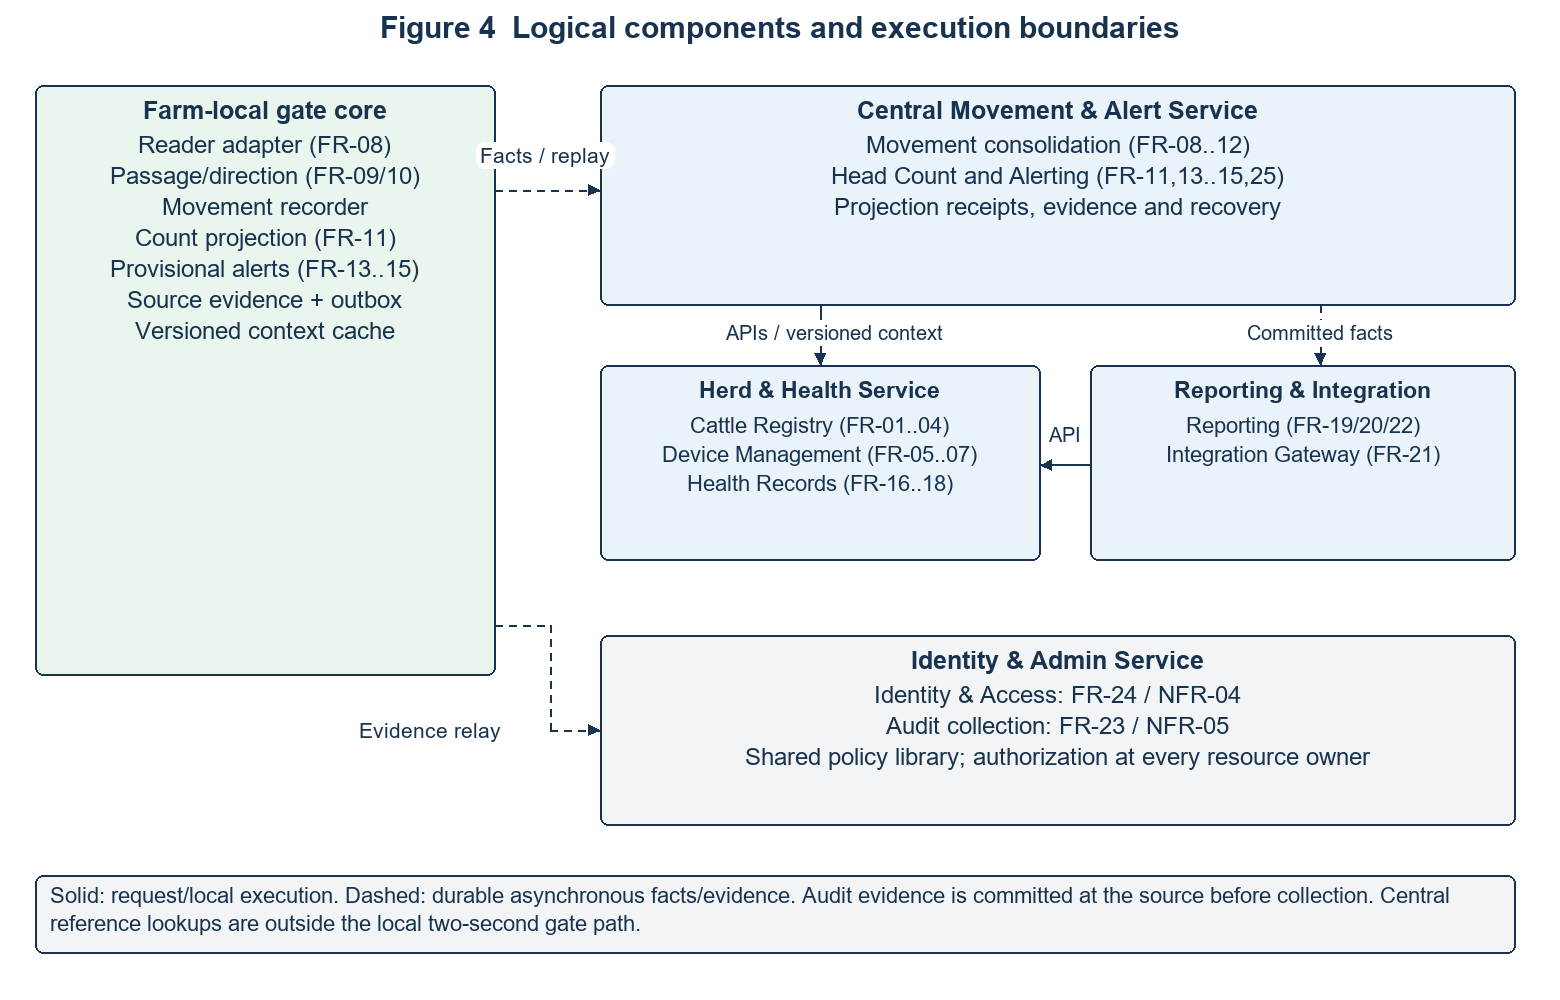
\includegraphics[width=\linewidth,height=0.42\textheight,keepaspectratio]{graphics/vinabeef/fig04-logical-components.png}
\caption{Logical components and farm/central execution boundaries}\label{fig:4}\end{figure}

\subsection{Physical Architecture}\label{sec:4.5}

\subsubsection{Step 1: Group components into deployable units}

Grouping follows criticality, data cohesion, rate of change and
location. The local gate core is placed at the farm; four coarse central
applications isolate domain work. Timing and resource behaviour of this
grouping are measured in M2.

{\small
\begin{longtable}[]{|>{\raggedright\arraybackslash}p{\dimexpr 0.3233\linewidth-2\tabcolsep\relax}|>{\raggedright\arraybackslash}p{\dimexpr 0.3233\linewidth-2\tabcolsep\relax}|>{\raggedright\arraybackslash}p{\dimexpr 0.3233\linewidth-2\tabcolsep\relax}|}
\hline
\textbf{Deployable unit} & \textbf{Components and data} & \textbf{Location / reason} \\ \hline
\endhead
Farm Edge Core & Reader adapter, passage/direction, local
movement/count, provisional alert rules, receipts/evidence/outbox,
caches & Three farm nodes; no central dependency for local outcome \\ \hline
Movement \& Alert & Central movement facts, count/alert projections,
projection receipts and outbox workers & Central; common movement domain
and recoverable projections \\ \hline
Herd \& Health & Cattle Registry, Health Records, Device Management &
Central; protected identity/custody/clinical ownership \\ \hline
Reporting \& Integration & Reports, export jobs, approved submission
intents/attempts & Central; isolate read-heavy and external work \\ \hline
Identity \& Admin & Identity, scoped grants, approved configuration,
protected Audit collection & Central; policy administration and evidence
collection \\ \hline
Web / supervisor clients & Presentation and scoped queries; farm-local
dashboard under lease & User devices; no authorization bypass \\ \hline
\end{longtable}
}

\subsubsection{Step 2: Define nodes and protections}

{\small
\begin{longtable}[]{|>{\raggedright\arraybackslash}p{\dimexpr 0.3233\linewidth-2\tabcolsep\relax}|>{\raggedright\arraybackslash}p{\dimexpr 0.3233\linewidth-2\tabcolsep\relax}|>{\raggedright\arraybackslash}p{\dimexpr 0.3233\linewidth-2\tabcolsep\relax}|}
\hline
\textbf{Node} & \textbf{Runtime and protection} & \textbf{Declared limitation} \\ \hline
\endhead
Farm x3 & Qualified readers; isolated LAN; small SSD/UPS edge server;
Docker Edge Core; local PostgreSQL & No destructive-storage zero-loss
guarantee; source evidence and history retained \\ \hline
Central & API gateway; four Spring Boot apps; three-node RabbitMQ quorum
cluster; PostgreSQL primary/synchronous standby; daily backup/WAL
archive & Service replicas do not remove shared DB/common infrastructure
failures; M2 qualifies resources \\ \hline
Clients & Browser and supervisor app; HTTPS; restricted farm-local
dashboard & New human logins and clinical/transfer/config writes remain
online-only \\ \hline
National system & External HTTPS API qualified during M2 & Receiver
semantics are outside VinaBeef control \\ \hline
\end{longtable}
}

Only the API gateway is publicly exposed for client traffic. Central
services/broker/stores remain private; farm edge links use assigned mTLS
machine identities. The gateway authenticates, while each owner checks
canonical resource permissions. Backup recovery and complete storage
loss require separately qualified RPO/RTO; the assignment no-loss
requirement is normal-operation preservation.

Farms reach the central site only through an IPsec site-to-site VPN.
Every farm-to-central connection is initiated by the edge: (1) AMQP
upload of committed facts, (2) HTTPS pull of versioned assignments and
devices, and (3) HTTPS refresh of configuration and policy leases, so
the design works behind farm NAT. An ops zone hosts the container
registry for signed edge images (staged rollout) and the monitoring and
log aggregation service. Each edge keeps its local history until the
central watermark confirms it, plus 90 days, before archiving. A failed
edge box is replaced from the registry image and local backup, and edge
recovery time is tested in M2. The baseline edge sizing is 4 vCPU, 8 GB
RAM and a 256 GB SSD.

\begin{figure}[htbp]\centering
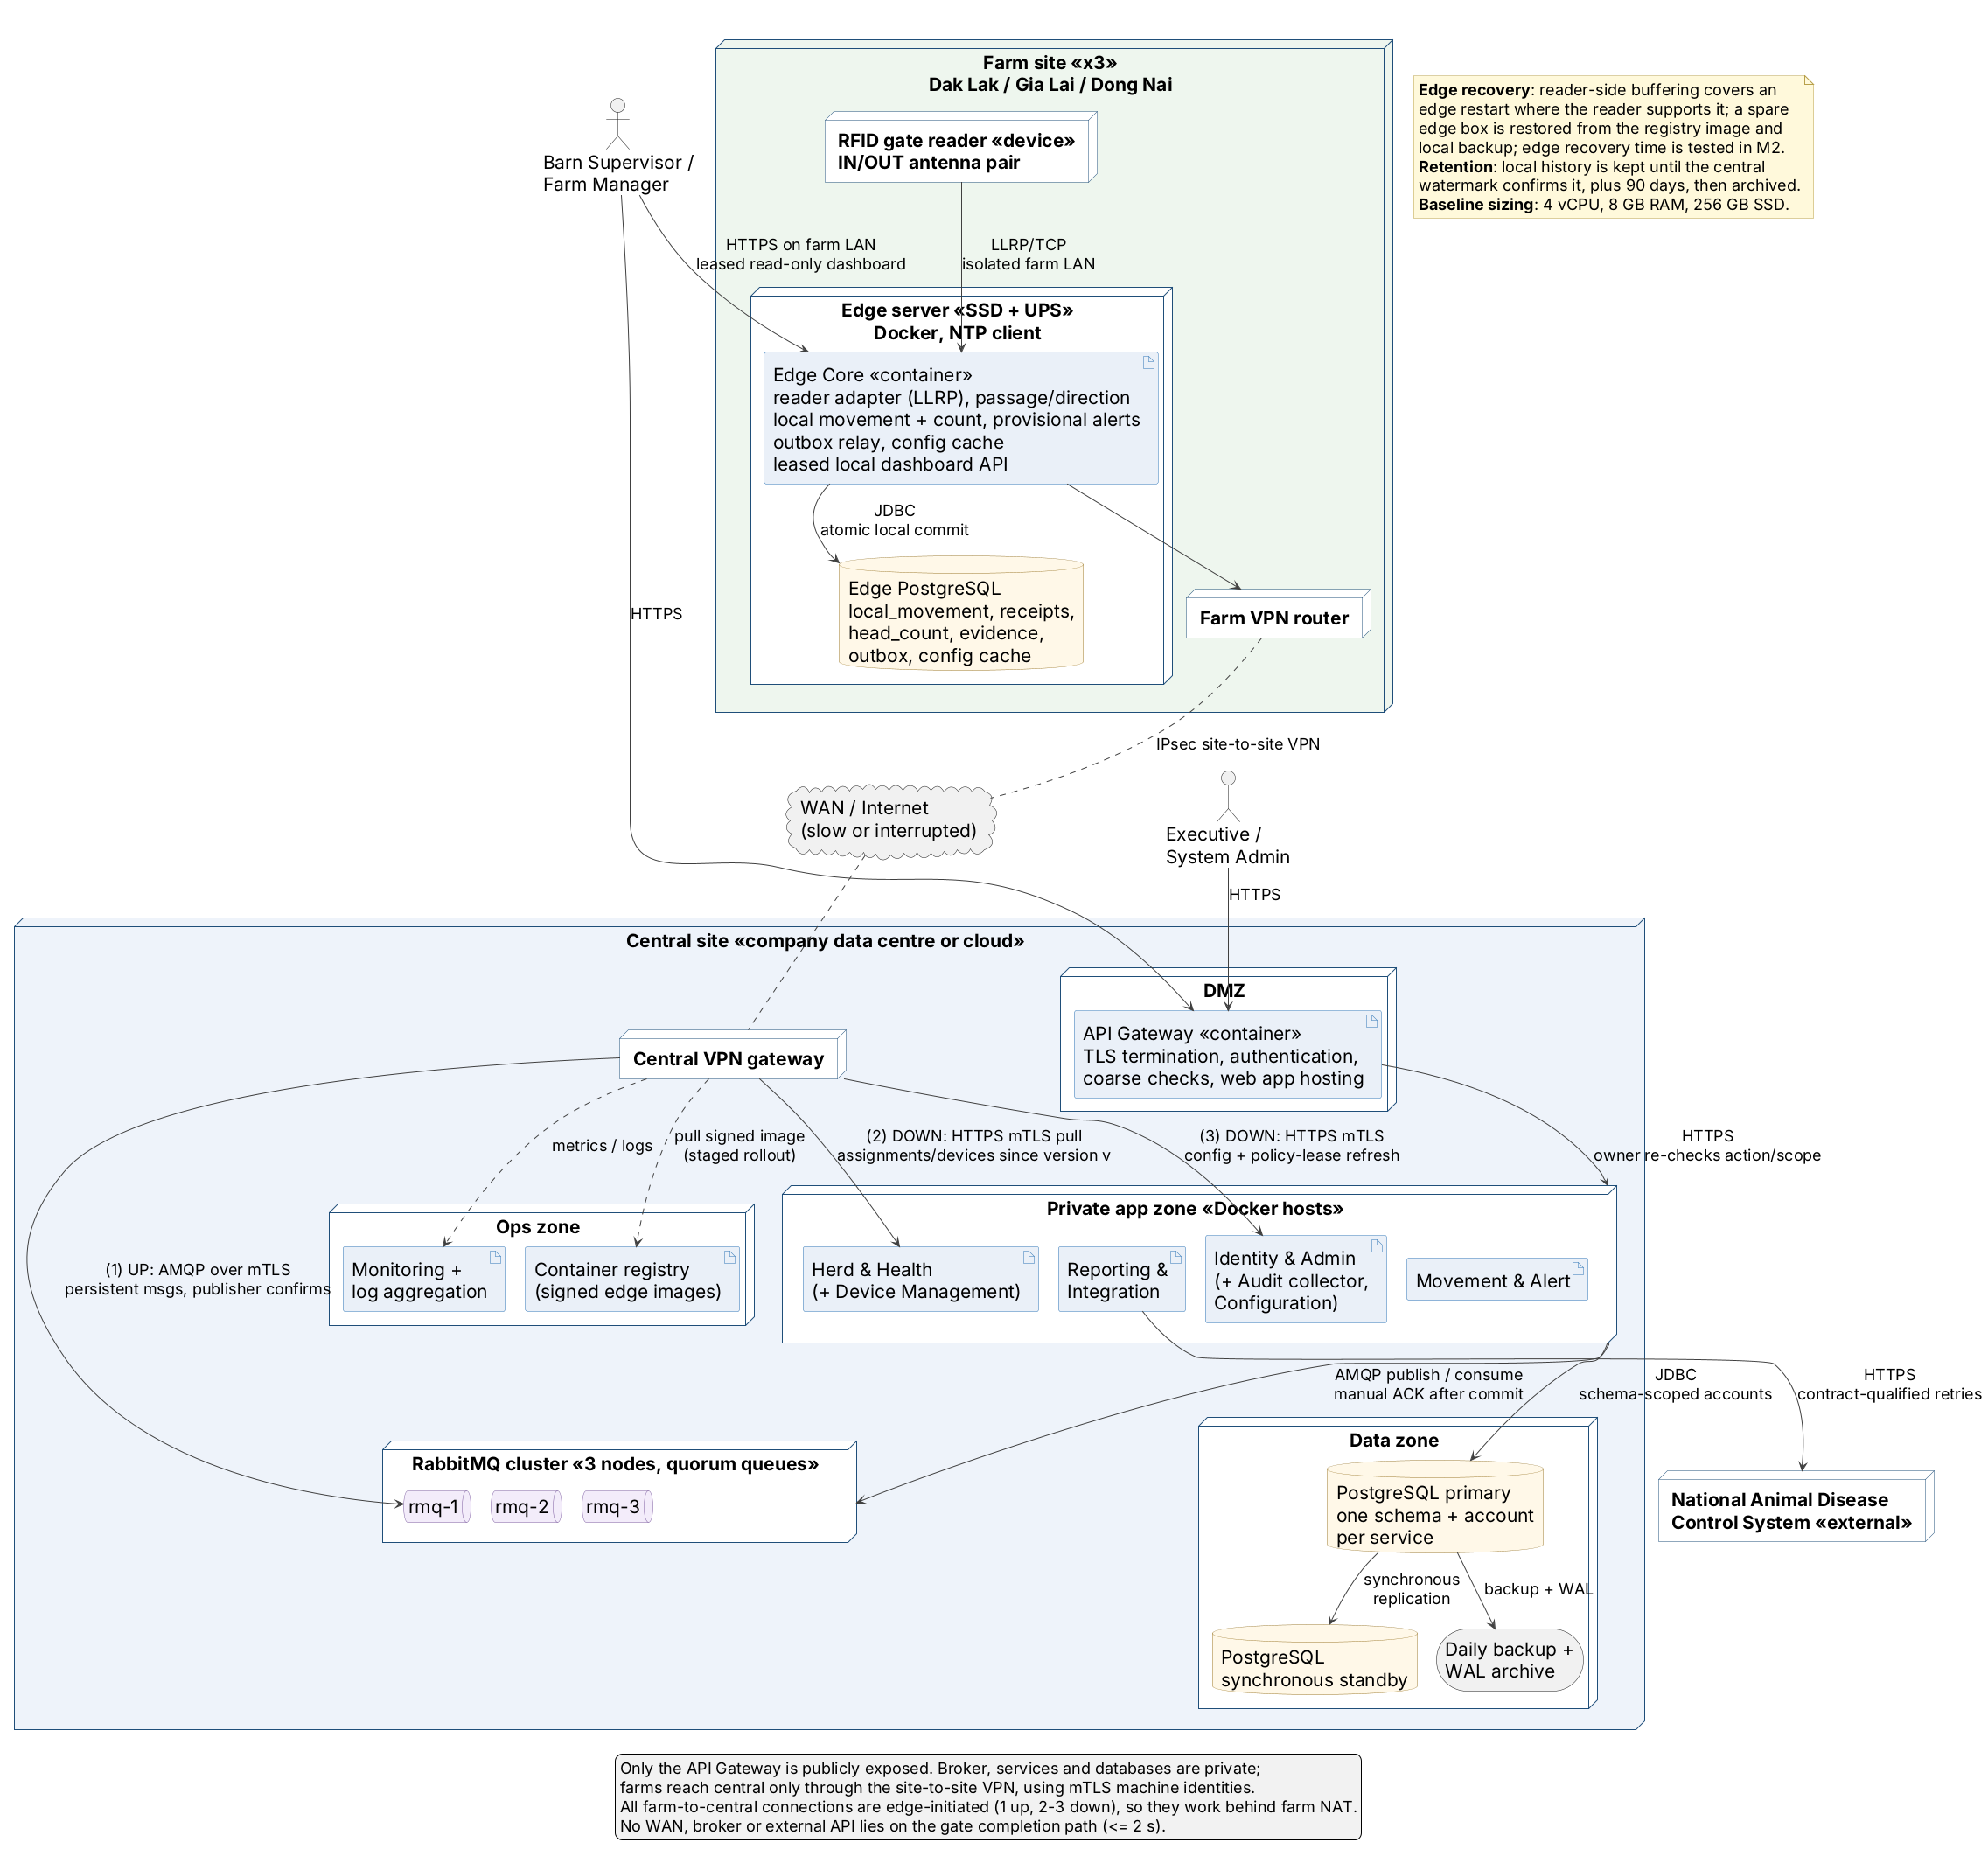
\includegraphics[width=\linewidth,height=0.8\textheight,keepaspectratio]{graphics/vinabeef/fig05-deployment.png}
\caption{Farm and central deployment with durable ownership}\label{fig:5}\end{figure}

\subsubsection{Step 3: Define communication and broker choice}

{\small
\begin{longtable}[]{|>{\raggedright\arraybackslash}p{\dimexpr 0.3233\linewidth-2\tabcolsep\relax}|>{\raggedright\arraybackslash}p{\dimexpr 0.3233\linewidth-2\tabcolsep\relax}|>{\raggedright\arraybackslash}p{\dimexpr 0.3233\linewidth-2\tabcolsep\relax}|}
\hline
\textbf{Link} & \textbf{Protocol} & \textbf{Completion semantics} \\ \hline
\endhead
Reader $\rightarrow$ Edge Core & Qualified LLRP/TCP farm-LAN adapter &
Source observations and application receipt semantics are established in
the reader contract \\ \hline
Edge $\rightarrow$ RabbitMQ $\rightarrow$ central & AMQP over
TLS/mTLS; persistent messages; quorum queues; publisher confirms; manual
consumer ACK & SENT\_TO\_BROKER proves broker receipt, not central
application completion \\ \hline
Client $\rightarrow$ owning service & Central HTTPS via gateway;
leased local HTTPS to farm Edge Core & Resource/approval checks at
service/query/export boundaries \\ \hline
Integration $\rightarrow$ external receiver & Qualified HTTPS API;
idempotency/status only if contract supports them & 202 remains pending;
unknown is retained; final evidence required \\ \hline
\end{longtable}
}

RabbitMQ is selected because this design needs durable work delivery,
per-consumer acknowledgements, redelivery and a stack the team can
configure and verify. The 200/1800 passage average is not a
raw-read/burst capacity bound. Kafka is a viable alternative for other
retention/replay or streaming needs; this project uses owned append-only
stores for history. Operational simplicity is a team assessment, not a
measured price comparison. M2 must qualify raw multiplicity, bursts,
concurrent farms, disk/CPU and recovery traffic.

\begin{figure}[htbp]\centering
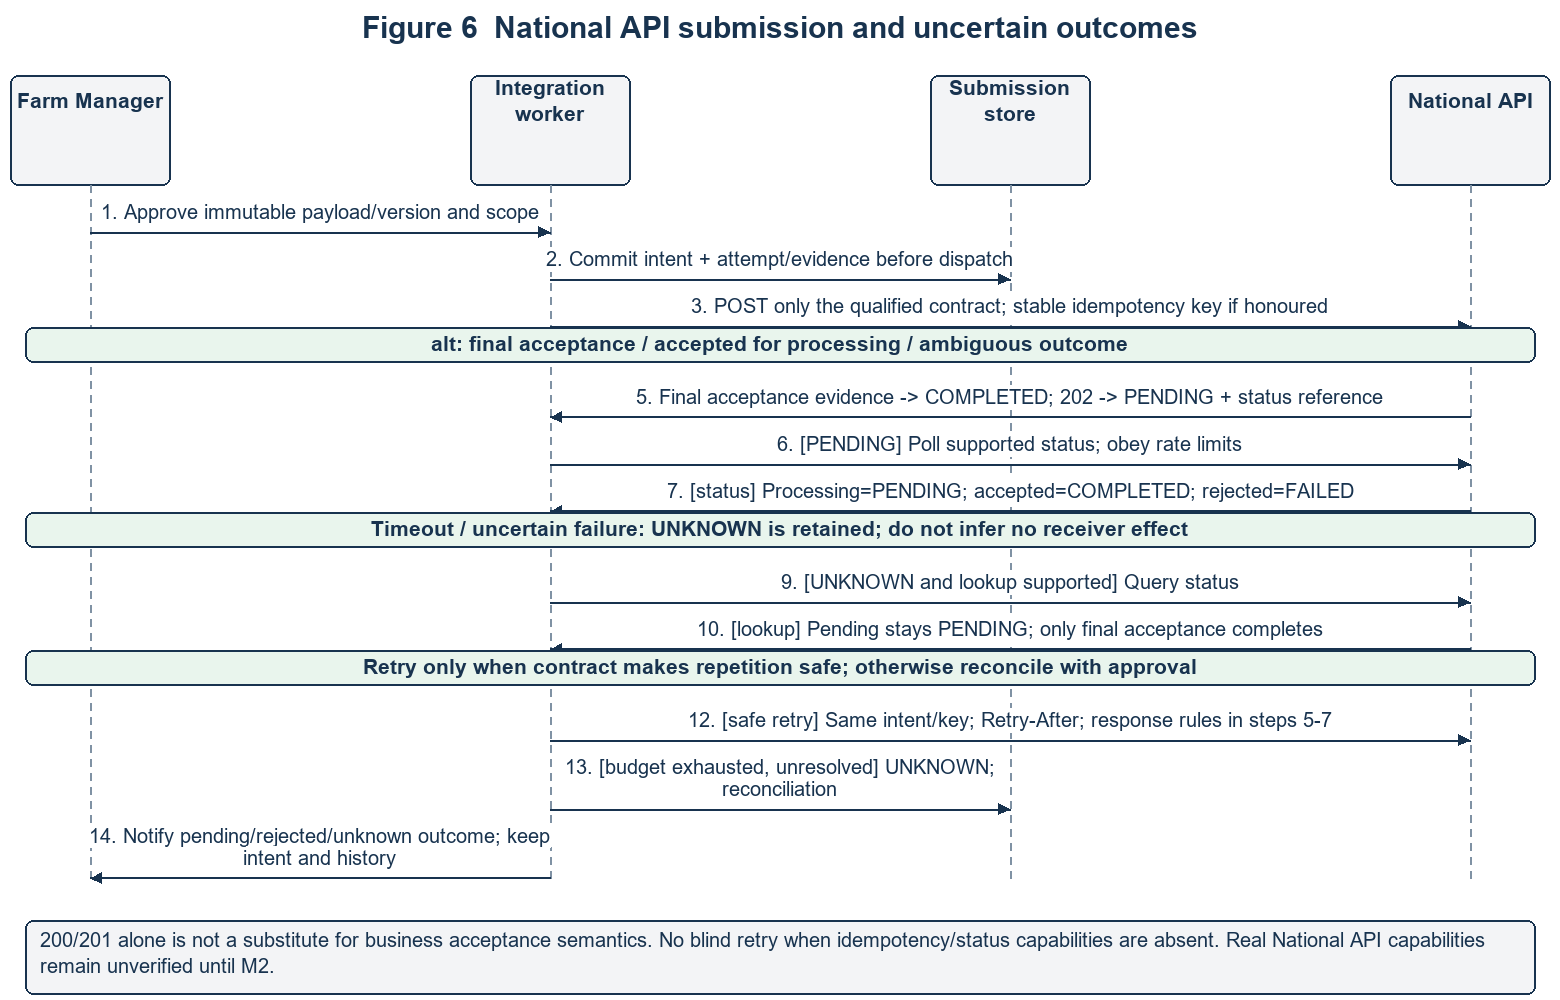
\includegraphics[width=\linewidth,height=0.42\textheight,keepaspectratio]{graphics/vinabeef/fig06-external-submission.png}
\caption{External submission with final acceptance and ambiguous-outcome handling}\label{fig:6}\end{figure}

\subsubsection{Step 4: Define owned data and domain invariants}

{\small
\begin{longtable}[]{|>{\raggedright\arraybackslash}p{\dimexpr 0.2904\linewidth-2\tabcolsep\relax}|>{\raggedright\arraybackslash}p{\dimexpr 0.2938\linewidth-2\tabcolsep\relax}|>{\raggedright\arraybackslash}p{\dimexpr 0.3858\linewidth-2\tabcolsep\relax}|}
\hline
\textbf{Store / owner} & \textbf{Data responsibilities} & \textbf{Write / recovery rule} \\ \hline
\endhead
Edge PostgreSQL / Edge Core & local\_movement; operation\_receipt;
local\_head\_count; source\_evidence; pending\_events outbox; versioned
assignment/config cache & Fact, effect, receipt and required evidence
commit atomically. SENT\_TO\_BROKER does not delete canonical local
history; duplicate/invalid dispositions remain durable. \\ \hline
Movement schema / Movement \& Alert & movement\_event;
processed\_event\_id; count/alert projections; projection receipts;
source\_evidence/outbox & Canonical facts append-only. Projection work
is durable and idempotent, with marker/effect/evidence committed per
projection owner. \\ \hline
Herd/Health schema & cattle permanentRFID; tag attachments/incidents;
devices; custody/transfer approvals; vaccination schedules and linked
clinical versions; receipts/evidence/outbox & Permanent RFID never
reassigned. Physical replacement preserves identity; different EPC is an
unapproved extension. Corrections append versions. \\ \hline
Reporting/Submission schema & report\_job; approved immutable
submission; payload hash/version; attempts; completion evidence &
Persist before dispatch; PENDING/UNKNOWN/COMPLETED/FAILED describe
business outcome. Unresolved exhaustion remains UNKNOWN. \\ \hline
Identity/Audit schema & human/machine principals; scoped RoleGrant;
policy version; protected audit\_record & No cross-service table access.
Canonical evidence is insert-only and references human or machine actor;
grants bind role and scope. \\ \hline
\end{longtable}
}

Stores may share the central PostgreSQL server, but accounts are limited
to owned schemas. Cross-owner access uses APIs/events and authorized
read models. Rebuild a projection only from a complete local history
plus its approved initial snapshot, or a verified central snapshot
merged with unsynchronized local facts. Compare equal source/event
watermarks first: ordinary eventual-consistency lag is not corruption.
Preserve original facts and evidence during reconciliation.

\begin{figure}[htbp]\centering
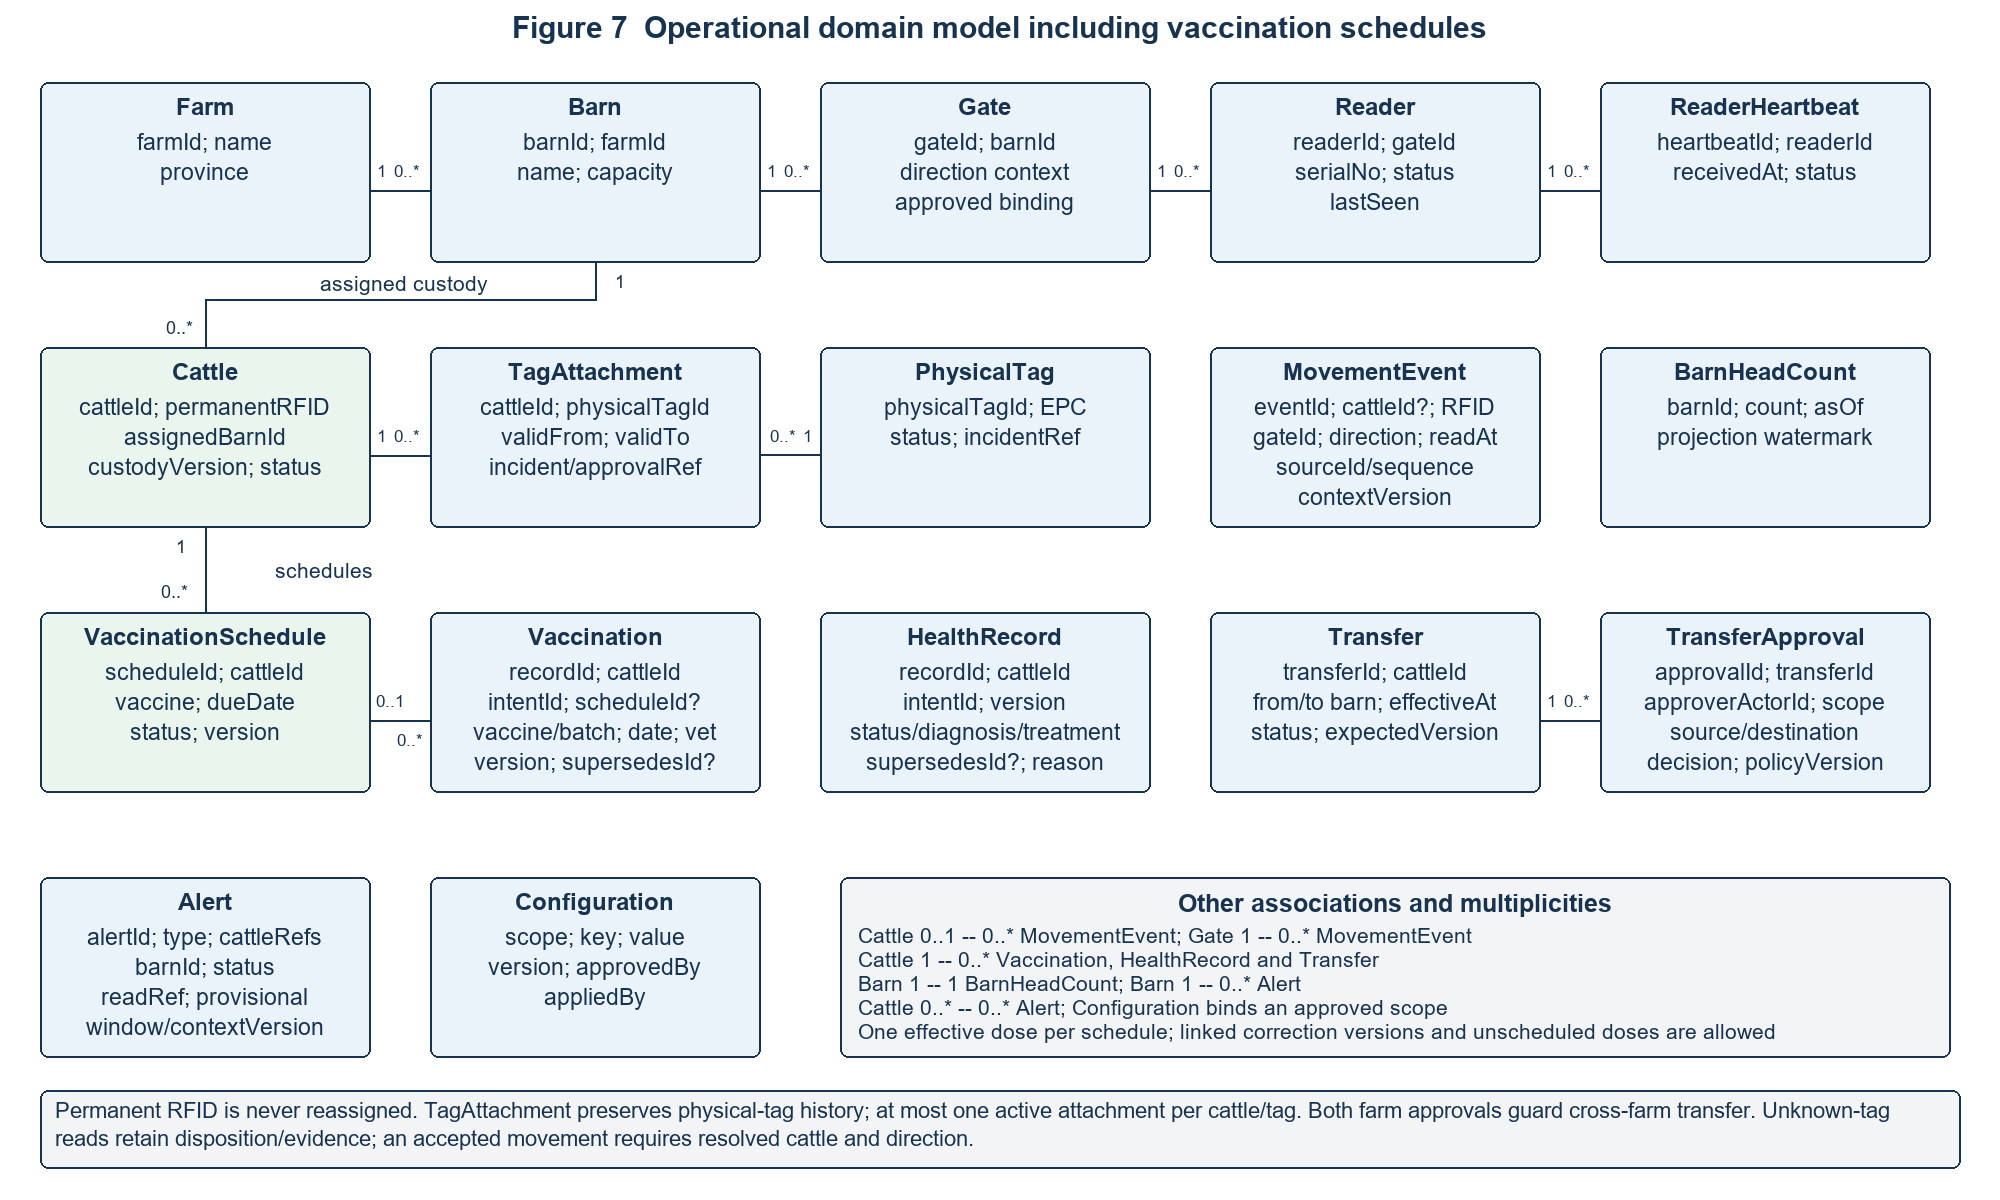
\includegraphics[width=\linewidth,height=0.42\textheight,keepaspectratio]{graphics/vinabeef/fig07-domain-entities.png}
\caption{Operational domain entities and immutable identity/custody constraints}\label{fig:7}\end{figure}

\begin{figure}[htbp]\centering
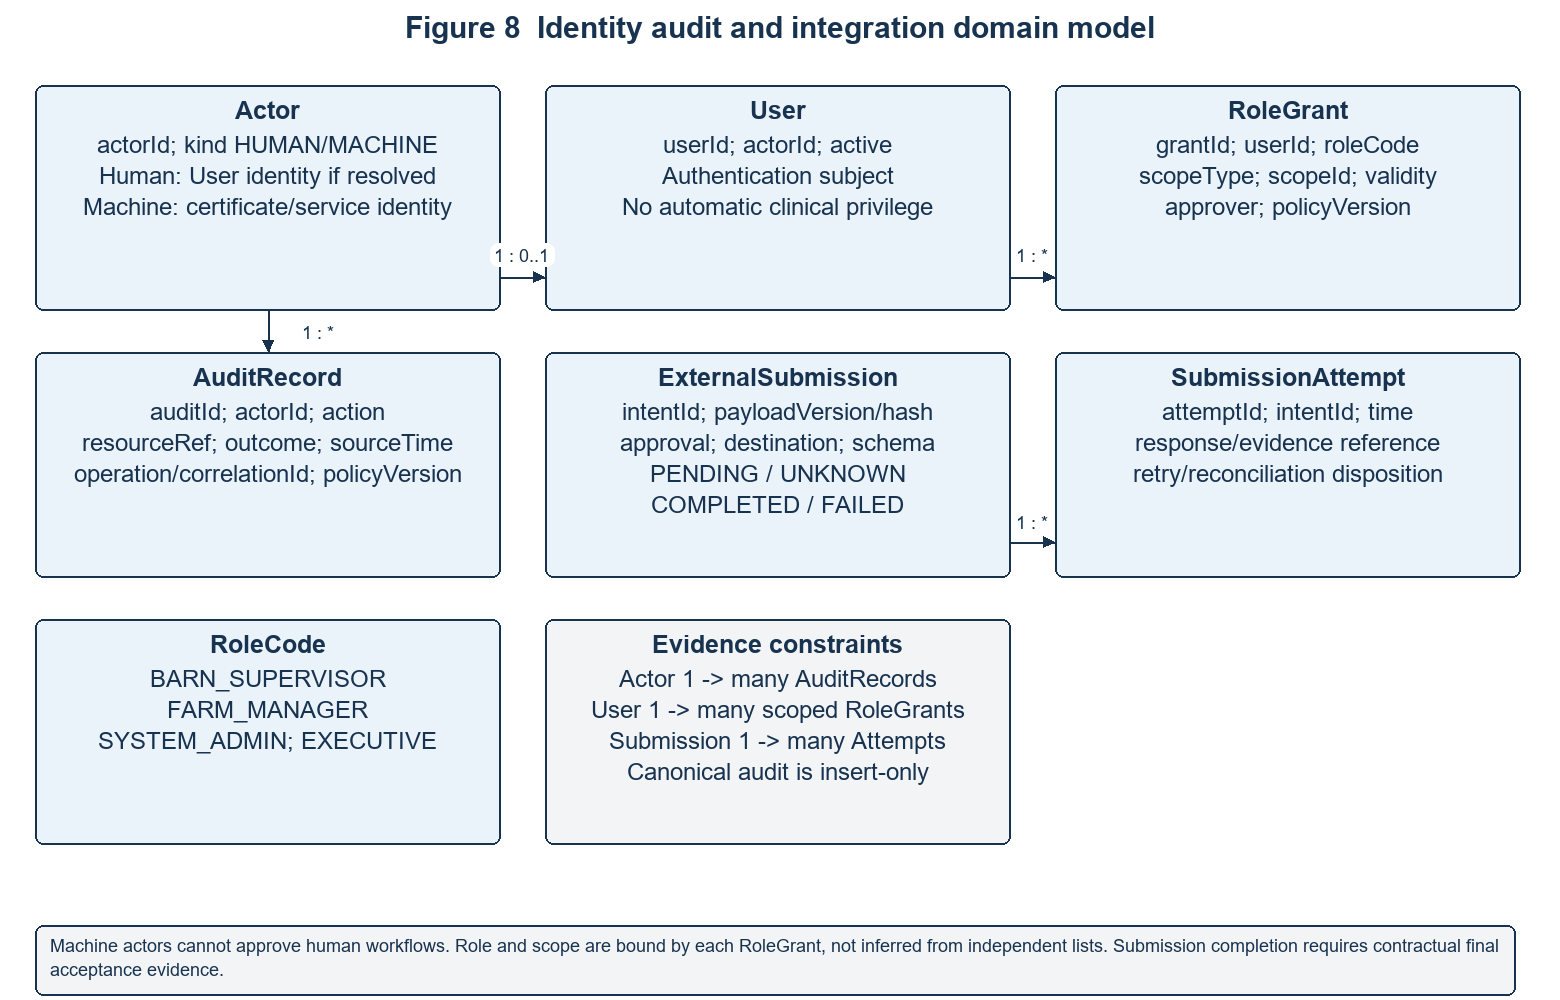
\includegraphics[width=\linewidth,height=0.42\textheight,keepaspectratio]{graphics/vinabeef/fig08-actors-grants.png}
\caption{Human/machine actors, scoped grants and external submission history}\label{fig:8}\end{figure}

\subsubsection{Step 5: Validate design walkthroughs and planned measurements}

Peak walkthrough: classify each qualified observation/passage and commit
the correct local disposition, movement/count effect and source evidence
within the SC-01 boundary. Raw-read bursts, source clock
uncertainty and resource limits are declared before M2 timing. Central
synchronization and the National API do not extend the local gate
critical path; placement alone is not a measured deadline guarantee.

Outage walkthrough: the gate core retains complete local facts,
receipts, count effects and evidence while context-dependent alerts are
provisional. Replay retains stable IDs and source sequence/event time;
late events cannot overwrite a newer state merely because they arrive
later. The 600-second recovery ends only when the outage cohort
is reconciled through central business facts, count/alert projections
and canonical evidence, while live local reads continue (SC-03).

Return-window walkthrough: match each OUT obligation with a later valid
IN and approved custody state; OUT/IN/OUT is missing again if its final
obligation remains open. BS acknowledgement and FM resolution are
distinct, audited actions. External walkthrough: final acceptance, 202,
rejection and timeout-after-effect have distinct outcomes; no
unsupported receiver capability is assumed.

\begin{figure}[htbp]\centering
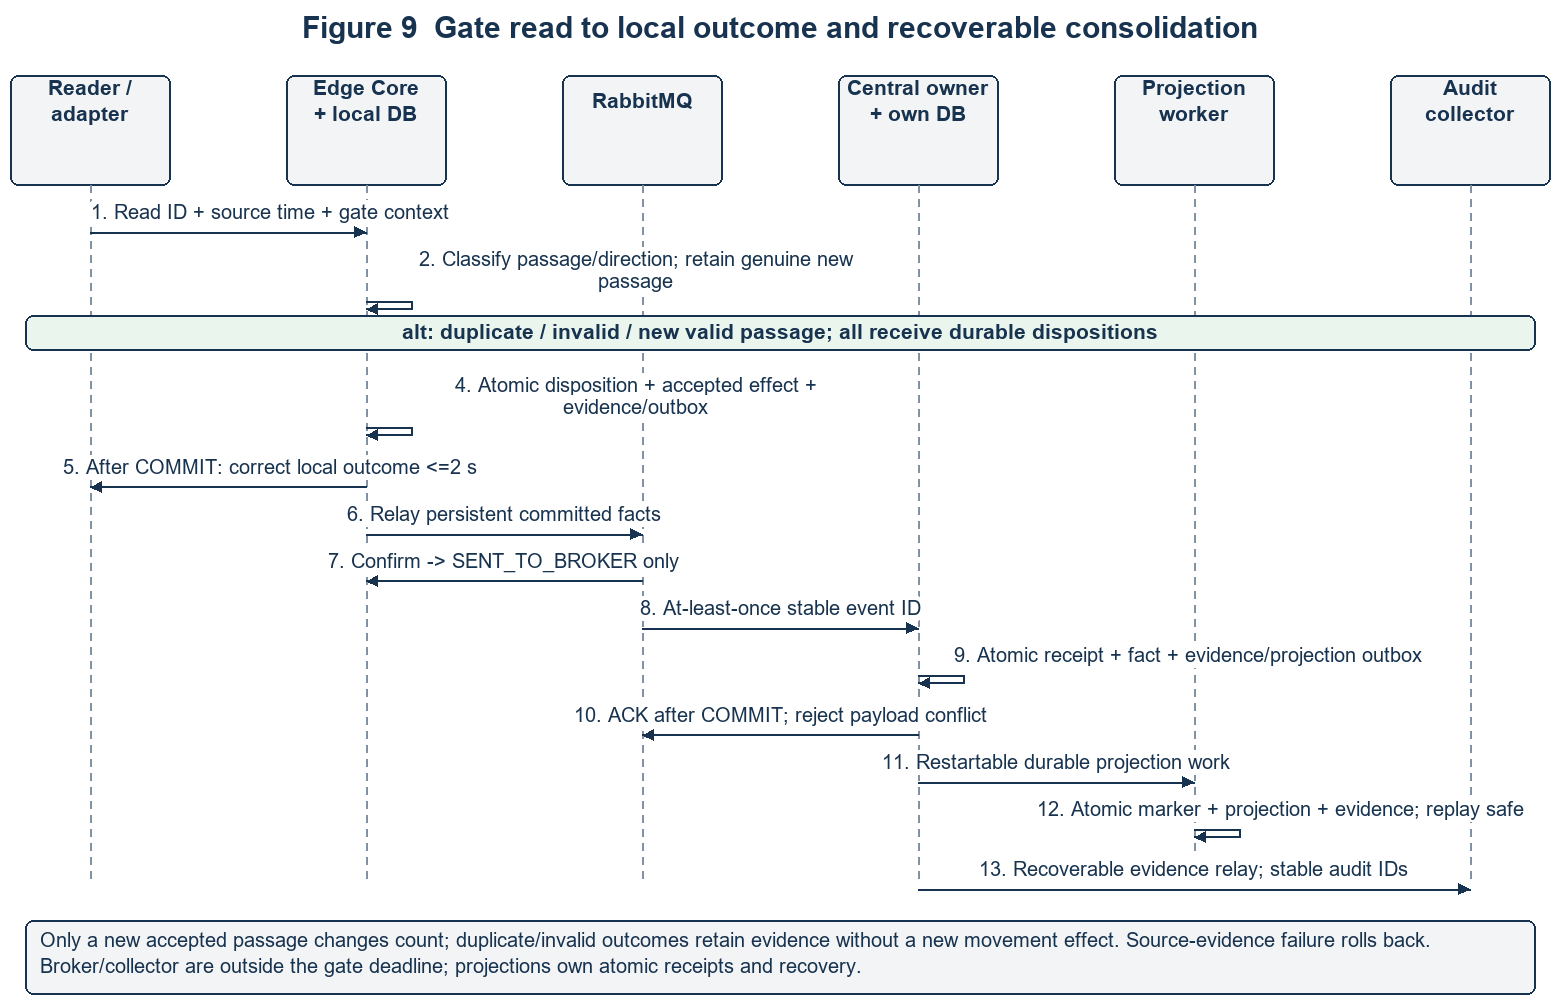
\includegraphics[width=\linewidth,height=0.42\textheight,keepaspectratio]{graphics/vinabeef/fig09-local-gate-outcome.png}
\caption{Durable local gate outcome and recoverable central projections}\label{fig:9}\end{figure}

\begin{figure}[htbp]\centering
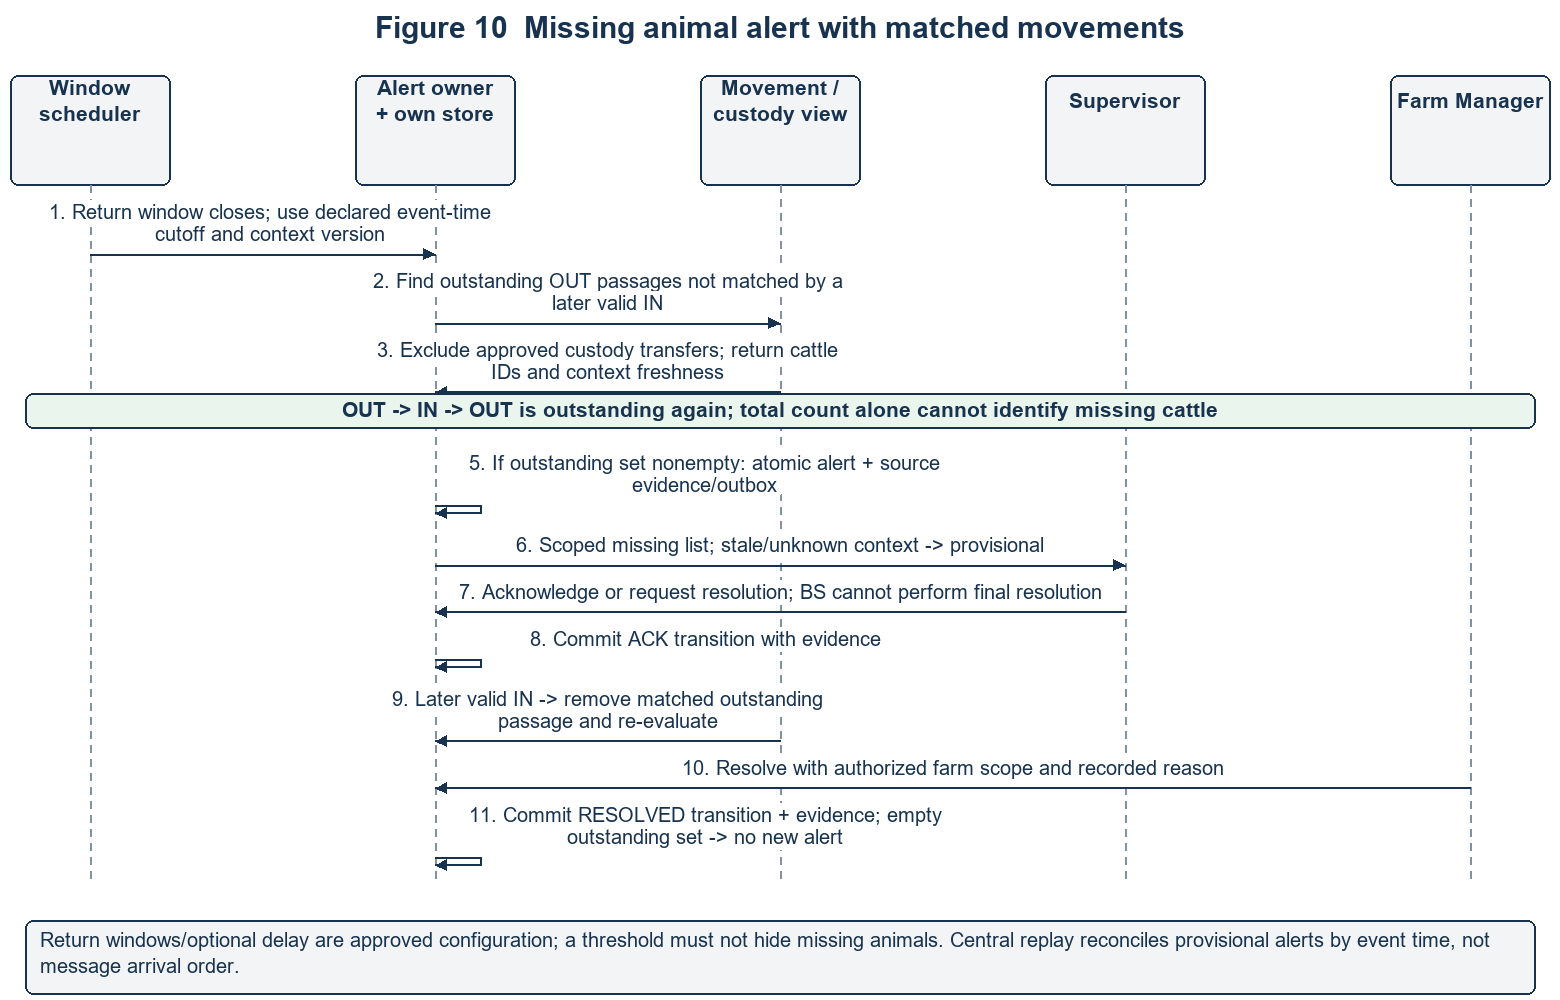
\includegraphics[width=\linewidth,height=0.42\textheight,keepaspectratio]{graphics/vinabeef/fig10-missing-detection.png}
\caption{Missing detection by outstanding movements and approved custody}\label{fig:10}\end{figure}

\begin{figure}[htbp]\centering
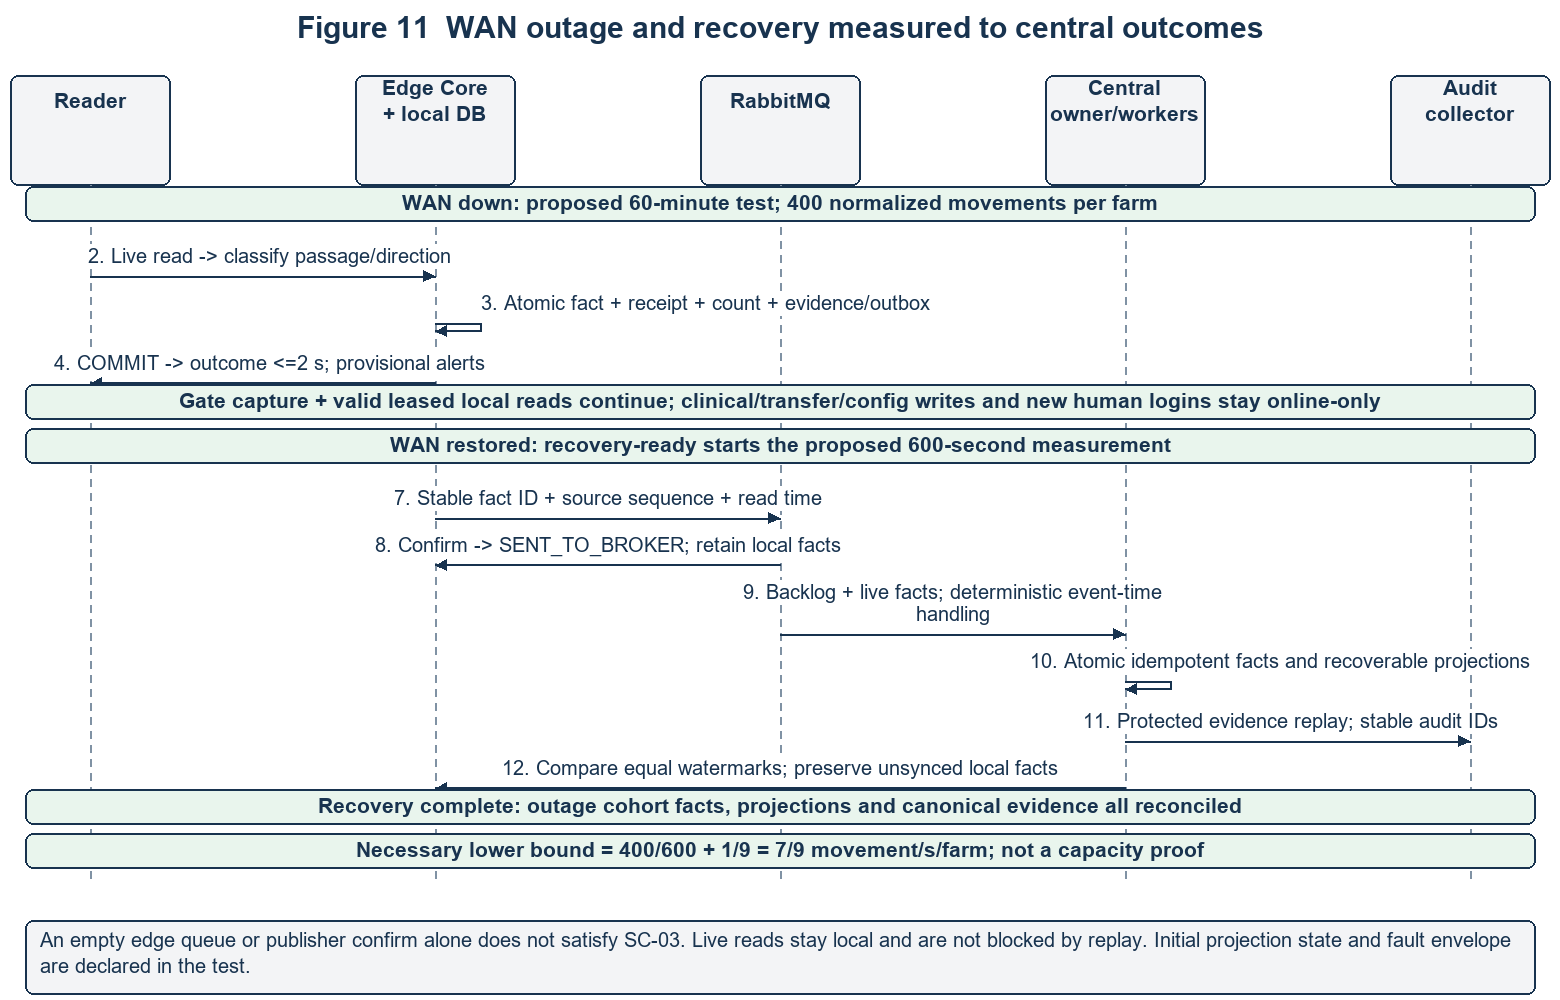
\includegraphics[width=\linewidth,height=0.42\textheight,keepaspectratio]{graphics/vinabeef/fig11-offline-capture.png}
\caption{Offline capture and recovery to completed central effects/evidence}\label{fig:11}\end{figure}

\section{Architecture Decisions}\label{sec:5}

Architecture decisions state the rules the system must follow. All
twelve ADRs below are accepted by the group; the Compliance line of each
ADR names the M2 scenarios and success criteria that verify it. Logical modules may share a
deployment unit or owned schema.

{\small
\begin{longtable}[]{|>{\raggedright\arraybackslash}p{\dimexpr 0.1355\linewidth-2\tabcolsep\relax}|>{\raggedright\arraybackslash}p{\dimexpr 0.6295\linewidth-2\tabcolsep\relax}|>{\raggedright\arraybackslash}p{\dimexpr 0.2050\linewidth-2\tabcolsep\relax}|}
\hline
\textbf{ADR} & \textbf{Rule} & \textbf{Drivers} \\ \hline
\endhead
ADR-01 & Service-based central backbone; committed gate facts are
propagated as events & D-01, D-02, D-03 \\ \hline
ADR-02 & Each farm runs an edge gateway; gate recording never depends on
the WAN or on central services & D-01, D-02 \\ \hline
ADR-03 & A read or a health write is acknowledged only after durable
commit; delivery to central is at-least-once & D-01 \\ \hline
ADR-04 & Every consumer and write path is idempotent on a stable
operation ID & D-01 \\ \hline
ADR-05 & Committed movement events and health records are never updated
or deleted; corrections are new linked records & D-01, D-03 \\ \hline
ADR-06 & Only the Integration Gateway calls external systems; ambiguous
outcomes are retried automatically only where the
receiver' s contract makes it safe & D-01 \\ \hline
ADR-07 & Central client traffic uses the API gateway; every owner checks
action/scope. Farm-local read-only access checks its existing session
and unexpired scoped lease. & D-03 \\ \hline
ADR-08 & Required audit evidence commits in the same transaction as the
change it records & D-03, D-01 \\ \hline
ADR-09 & No service reads or writes another service' s
tables & --- \\ \hline
ADR-10 & Spring Boot, PostgreSQL, RabbitMQ, Docker & D-01 \\ \hline
ADR-11 & A gate read completes at the farm edge; central services
consolidate & D-02, D-01 \\ \hline
ADR-12 & During WAN loss, gate capture and valid leased local reads
continue; clinical, transfer and configuration writes and new human
logins remain online-only & D-03, D-01 \\ \hline
\end{longtable}
}

\subsection{ADR-01: Service-based backbone with event-driven gate processing}\label{adr:01}

\textbf{Status: Accepted.}

\textbf{Context:} The driving characteristics are D-01
Reliability/Durability, D-02 Performance and D-03 Security/Auditability
(\Cref{sec:3.3}). The average gate rate is low, about 0.11 passages per
second per farm (\Cref{sec:2.2.1}), but reads arrive in bursts and each
read carries its own two-second deadline. The system serves three farms
and is built by a small team, so operational cost is a constraint.

\textbf{Decision:} The central system is four coarse-grained services
--- Movement \& Alert, Herd \& Health, Reporting \& Integration,
Identity \& Admin (\Cref{sec:4.5}) --- behind an API gateway. After the farm edge commits a gate outcome (ADR-11),
the committed facts travel as events through a message broker to the
central services. Nothing on the gate path
waits on a synchronous call to a central service.

\textbf{Consequences: Separate process/deployment boundaries can isolate
movement from reporting and external workers. The shared central DB is
still a common fault domain. This is fewer service units than the
fine-grained V6 variant; operational cost is an assessment to verify,
not a measured fraction.}

\textbf{Compliance:} QAS01 (two-second gate outcome under the peak
workload) and QAS03 (crash and replay). Architecture review: no
synchronous dependency from the gate path to a central service.

\subsection{ADR-02: Edge gateway per farm}\label{adr:02}

\textbf{Status: Accepted.}

\textbf{Context:} Farms are rural and the WAN link may be slow or
interrupted (\Cref{sec:1.5}), yet no movement may be lost and every read
has a two-second deadline.

\textbf{Decision:} Each farm runs an edge server (local SSD, UPS, local
PostgreSQL) that receives reader events over LLRP on the farm LAN and
forwards events to the central broker over AMQP with mTLS. What the edge
completes locally is fixed by ADR-11; what it may do offline is fixed by
ADR-12.

\textbf{Consequences:} Farms keep recording through WAN outages, and WAN
latency is off the gate path. Edge software must be deployed, monitored
and updated at three sites, and each edge needs its own machine
identity.

\textbf{Compliance:} QAS02 (60-minute WAN outage with no lost or
duplicated movements).

\subsection{ADR-03: Persist before acknowledge, at-least-once delivery}\label{adr:03}

\textbf{Status: Accepted.}

\textbf{Context:} No movement or health record may be lost in normal
operation (NFR-02).

\textbf{Decision: Each owner atomically commits its effect, stable
operation receipt and required source evidence/outbox before success or
message ACK. Edge relay status becomes SENT\_TO\_BROKER only after
publisher confirm; local canonical facts/evidence remain retained.
Central consumers ACK after their owned transaction; durable projection
outboxes are drained by restartable idempotent workers. Broker receipt,
consumer fact commit, projection completion and canonical audit
collection are distinct stages.}

\textbf{Consequences:} No loss within the declared fault envelope, but
duplicates are possible; ADR-04 makes them harmless. A broker confirm
alone does not prove that the business effect was applied.

\textbf{Compliance:} QAS03 (crash after commit, before acknowledgement);
SC-02.

\subsection{ADR-04: Idempotent consumers and write paths}\label{adr:04}

\textbf{Status: Accepted.}

\textbf{Context:} At-least-once delivery, client retries and RFID
multi-reads all produce duplicates.

\textbf{Decision: Every normalized movement and health intent has a
stable ID; each effect owner commits its processed
marker/effect/evidence atomically. Same ID/different content is
rejected. Physical passage classification uses qualified observation
identity, gate/antenna context and direction state; repeated
observations of one passage are collapsed, while a genuine OUT/IN
sequence within the observation window creates two movements. Transport
retries preserve the original event ID.}

\textbf{Consequences:} Correct counts and a single treatment record
despite retries; each consumer needs a processed-ID store.

\textbf{Compliance: QAS03 (exactly 100 effects from replayed IDs); QAS05
(one health intent); additional passage fixture: OUT then IN within the
observation window yields two logical movements and the correct count.}

\subsection[ADR-05: Append-only movement events and versioned health records]{ADR-05: Append-only movement events and versioned\\ health records}\label{adr:05}

\textbf{Status: Accepted.}

\textbf{Context:} Movement and health history must be complete and
trustworthy, and head counts must be explainable.

\textbf{Decision: Committed movement, health and audit facts are not
updated or deleted. Movement correction appends a compensating event;
health correction appends a linked version. Canonical permanent RFID is
never reassigned, and tag incidents preserve the cattle history; a
different RFID requires a separately approved extension. Counts are
rebuildable projections with declared initial state and watermarks.
Application accounts cannot UPDATE/DELETE canonical fact/evidence
tables; mutable operational projections and dispatch status are
separate.}

\textbf{Consequences:} Full history and rebuildable counts. Storage
grows over time, and queries must select the current version.

\textbf{Compliance:} SC-02 and SC-05; database-permission check in M2.

\subsection{ADR-06: Single integration point with safe external delivery}\label{adr:06}

\textbf{Status: Accepted.}

\textbf{Context:} The National Animal Disease Control System is outside
VinaBeef' s control. Its failures must not affect core
functions, and a timeout can follow a side effect at the receiver.
Whether its API supports idempotency keys or status lookup is not yet
known.

\textbf{Decision: Only Integration Gateway calls external systems.
Persist the approved immutable intent/payload version before dispatch.
Final contractual business acceptance evidence is required for
COMPLETED; 202 or a found-but-processing status is PENDING. An ambiguous
outcome remains UNKNOWN. Retry only when an honoured idempotency
contract or conclusive status semantics establishes safety; lookup
absence/404 is not automatically proof of no receiver effect. Back off,
respect applicable Retry-After, bound attempts, and retain unresolved
exhausted work for FM-approved reconciliation. Confirmed rejection is
FAILED; retry exhaustion alone does not prove rejection.}

\textbf{Consequences:} External changes are contained in one component,
and no submission is lost or blindly duplicated. Some submissions may
wait for manual reconciliation. The real API contract must be qualified
during M2.

\textbf{Compliance:} QAS06; SC-06.

\subsection{ADR-07: API gateway with service-level authorization}\label{adr:07}

\textbf{Status: Accepted.}

\textbf{Context:} RBAC must apply to every request, and permissions
depend on barn and farm scope (\Cref{sec:2.2.3}), which only the service
that owns a resource can evaluate.

\textbf{Decision: Central client traffic enters through the API gateway,
which authenticates users (JWT). Every resource owner checks action and
canonical barn/farm scope at service, query and export boundaries;
unspecified actions are denied. The farm-LAN read-only dashboard is the
declared exception: Edge Core validates its existing session, cached
scoped grant and unexpired policy lease on every local request (\Cref{sec:2.2.2}; ADR-12). It cannot authorize online-only actions or a new human
login. Readers and workers use separate provisioned machine identities
and cannot act as human approvers.}

\textbf{Consequences:} Consistent, layered security. Authorization logic
runs in every service, so it is packaged as a shared library and policy
versions are audited. The gateway must be highly available.

\textbf{Compliance:} QAS04 (wrong-farm access, SA clinical write and
revoked export are all denied); SC-04.

\subsection{ADR-08: Audit evidence in the same transaction}\label{adr:08}

\textbf{Status: Accepted.}

\textbf{Context:} Comprehensive audit logging is mandatory (NFR-05), and
evidence written after the fact can be lost.

\textbf{Decision:} Each covered operation writes its audit evidence to
an outbox in the same database transaction as the change, and a relay
publishes it to the insert-only audit store. Coverage includes state
changes, sensitive reads (clinical profiles, exports, audit evidence)
and authorization denials (\Cref{sec:2.2.4}). If mandatory evidence cannot
be written, the operation does not report success. A denial stays denied
even if its log write fails, and the gap is recorded. Relay duplicates
keep their audit ID and are de-duplicated.

\textbf{Consequences:} No audited business success without its evidence,
at a small write cost. The edge store also needs an outbox for gate
evidence.

\textbf{Compliance:} QAS05 (a health write whose evidence step fails is
rolled back); SC-05.

\subsection{ADR-09: No shared tables between services}\label{adr:09}

\textbf{Status: Accepted.}

\textbf{Context:} Services must be able to change their data models
independently.

\textbf{Decision:} Each service owns one PostgreSQL schema. Services
exchange data only through APIs or events, even on a shared database
server; data another service needs is copied into a read model.

\textbf{Consequences:} Looser coupling and independent schema change.
Some data is duplicated, and read models are eventually consistent.

\textbf{Compliance:} Each service' s database account
holds grants on its own schema only; checked in M2.

\subsection{ADR-10: Technology stack}\label{adr:10}

\textbf{Status: Accepted.}

\textbf{Context: The team works with Java and Spring Boot, and M2
requires implementation and testing. The average passage rate is low,
but it does not bound raw-read bursts. The per-read deadline and
preservation of movement/health records remain mandatory.}

\textbf{Decision: Use Spring Boot, owned PostgreSQL schemas/local
stores, RabbitMQ quorum queues with confirms/manual ACK, and Docker. Broker choice follows delivery/recovery needs and
team familiarity, not the passage average alone. Kafka remains an
alternative for different stream-retention needs. M2 qualifies bursts,
raw reads, resource configuration and operational complexity (\Cref{sec:4.5}).}

\textbf{Consequences:} Mature, documented tools and one stack at edge
and centre. Replaying long histories relies on the append-only tables
(ADR-05) rather than on broker retention.

\textbf{Compliance:} M2 build and deployment configuration.

\subsection{ADR-11: Gate processing completes at the farm edge}\label{adr:11}

\textbf{Status: Accepted.}

\textbf{Context:} Each read must complete within two seconds (NFR-01)
and survive WAN outages (NFR-02, NFR-03). If completion depends on
central services, the deadline includes WAN latency and fails whenever
the link is down.

\textbf{Decision: Edge Core runs qualified reader/passage/direction
logic, local movement/count and provisional alerts against versioned
cached context. A required read completes at a durable correct local
disposition: accepted movement/count/evidence, or duplicate/invalid
disposition with its required evidence. The central Movement \& Alert
application consolidates facts and recoverable projections. Compare
equal source/event watermarks before detecting divergence. Rebuild from
complete retained local facts plus approved initial snapshot, or a
verified snapshot merged with unsynced local facts; never discard
pending history or treat ordinary sync lag as corruption.}

\textbf{Consequences: The gate completion path has no central
dependency. Edge and central share a versioned rule module; cache
versions and source sequence/event time make replay and
provisional-alert reconciliation explainable. Cached context can be
stale, so domain conclusions remain provisional until reconciliation;
actual timing is verified in M2.}

\textbf{Compliance:} QAS01 (timing measured to the edge commit); QAS02;
SC-01, SC-03.

\subsection{ADR-12: Offline operation scope}\label{adr:12}

\textbf{Status: Accepted.}

\textbf{Context:} During a WAN outage the edge cannot validate central
policy, and clinical and transfer operations need current custody and
approvals (\Cref{sec:2.2.2}).

\textbf{Decision:} Offline, the edge runs gate capture, local movement
and head count, alert evaluation with cached context, and durable
pending synchronization. Clinical writes, transfers, configuration
changes and new human logins are online-only. Existing local dashboard
sessions expire 15 minutes after the last central policy
validation.

\textbf{Consequences: Gate capture continues with its separate machine
identity, while human writes and new logins remain denied offline. A
centrally revoked grant cannot be observed immediately during WAN loss;
the local read-only lease bounds stale permission to 15 minutes, or earlier session expiry. The group accepts this trade-off:
continuous gate capture is worth a bounded window of stale read-only
access. Health events occurring during an outage are entered after
recovery.}

\textbf{Compliance:} QAS02 (local processing continues); QAS04
(online-only actions are denied).

\section{Design Principles}\label{sec:6}

Design principles are guidelines for developers. Unlike architecture
decisions, they guide judgement rather than impose a rule.

\subsection{SOLID Principles}\label{sec:6.1}

{\sloppy The table names the classes in the repository that apply each principle
(modules \texttt{herd-health}, \texttt{access-policy} and
\texttt{farm-edge} under \texttt{backend/}). \Cref{sec:m2-health-solid} explains the
Health authorization slice in more detail. The M1 report used
design-level names (\texttt{MovementRecorder}, \texttt{HeadCountCalculator},
\texttt{AlertRule}, \texttt{ReportExporter}, \texttt{ReaderEventSource},
\texttt{ReaderHealthMonitor}); the M2 prototype does not implement them, so
they are replaced here by the classes that exist.\par}

{\small
\begin{longtable}[]{|>{\raggedright\arraybackslash}p{\dimexpr 0.2280\linewidth-2\tabcolsep\relax}|>{\raggedright\arraybackslash}p{\dimexpr 0.5092\linewidth-2\tabcolsep\relax}|>{\raggedright\arraybackslash}p{\dimexpr 0.2328\linewidth-2\tabcolsep\relax}|}
\hline
\textbf{Principle} & \textbf{Application in VinaBeef (code)} & \textbf{Supports} \\ \hline
\endhead
Single Responsibility & \texttt{HealthController} handles HTTP only;
\texttt{HealthIntentService} runs the use cases; \texttt{HealthAuthorization}
applies the authorization decision order; \texttt{JdbcHealthRepository}
owns the SQL. At the farm edge, \texttt{PassageClassifier} is a pure
classification rule (no Spring, no database) and \texttt{GateService} owns
the transaction. & NFR-08 \\ \hline
Open/Closed & A new identity or grant source is a new bean behind
\texttt{TrustedPrincipalProvider} or \texttt{CurrentGrantContextProvider};
\texttt{HealthBoundaryConfiguration} registers fail-closed defaults with
\texttt{@ConditionalOnMissingBean}, so the use cases do not change. &
NFR-04, NFR-08 \\ \hline
Liskov Substitution & Every \texttt{CurrentGrantContextProvider} (the JSON
fixture \texttt{JsonFixtureCurrentGrantContextProvider} and the fail-closed
default) either returns the grant context for the verified subject or fails
as unavailable; an unavailable source never yields an allow. & NFR-04 \\ \hline
Interface Segregation & Five inbound ports: \texttt{LookupCattleUseCase},
\texttt{SubmitHealthIntentUseCase}, \texttt{GetHealthIntentReceiptUseCase},
\texttt{GetHealthHistoryUseCase}, \texttt{ListCattleInScopeUseCase}; a
client such as \texttt{HealthController} depends only on the operations it
calls. & NFR-08 \\ \hline
Dependency Inversion & \texttt{HealthIntentService} depends on
\texttt{HealthRepository}, implemented by \texttt{JdbcHealthRepository};
\texttt{HealthAuthorization} depends on \texttt{AccessPolicyPort},
implemented by \texttt{ClinicalAuthorizationPolicyAdapter}, which calls
\texttt{ClinicalAuthorizationPolicy} in \texttt{libs/access-policy} (plain
Java, no Spring). & NFR-04, NFR-08 \\ \hline
\end{longtable}
}

\subsection{Other Principles}\label{sec:6.2}


\begin{itemize}
  \item Complete at the edge, consolidate at the centre: nothing on the gate path waits on the WAN (ADR-02, ADR-11).
  \item Persist, then acknowledge: never report success for work that is not durably committed (ADR-03).
  \item Assume duplicates: any message or request may arrive more than once; never assume a remote receiver is idempotent unless its contract says so (ADR-04, ADR-06).
  \item Deny by default, least privilege: each role, service and machine identity gets only the permissions it needs (ADR-07).
  \item Evidence with the change: an audited operation and its evidence commit together (ADR-08).
  \item Loose coupling, high cohesion: communicate through events and versioned APIs; keep logic that changes together in one service (ADR-09).
  \item Observability: structured logs, metrics and reader heartbeats; every log and audit record carries an operation or correlation ID.
  \item Keep it simple: add a service or a technology only when a driving characteristic requires it.
\end{itemize}

\subsection{Applied SOLID in Health Authorization}\label{sec:m2-health-solid}

\textbf{Single Responsibility.} The Java policy evaluates grants against
the action and resource supplied by Health. The application service
enforces the decision and coordinates acceptance, retry and audit
evidence within the Health transaction. A change to a scope rule can
be exercised in policy tests. A change to storage or transaction
behavior is exercised through the Health backend.

\textbf{Dependency Inversion.} Health's application layer calls
\texttt{AccessPolicyPort}. The concrete adapter maps Health's principal,
grant and resource types to the library. The policy rules are testable
without Spring or PostgreSQL. Running the integrated slice verifies
that the adapter supplies the right context and Health enforces the
decision. \Cref{sec:m2-health-auth,sec:m2-health-results} describes both
levels of verification.

\subsection{Reflection on the Health Slice}\label{sec:m2-health-reflection}

The PostgreSQL suite exposed a failure that the policy unit tests could
not exercise. The JDBC driver could not bind a Java \texttt{Instant}
directly to a timestamp parameter during a clinical write. Converting
the timestamp to an offset date-time at the JDBC boundary preserved
the domain model and the authorization contract. The rollback test
also checks that its exception came from the injected source-evidence
insert failure before it checks the database state. That assertion
matters because an unrelated error early in the write could also
leave zero rows. These two checks show why policy unit tests and
database integration tests both belong in the verification plan.

\section{Traceability}\label{sec:7}

Each requirement is traced to the logical components of \Cref{sec:4.4}, the
decisions of \Cref{sec:5}, and its verification criteria: a use case of \Cref{app:A}
or an acceptance-criteria group of \Cref{sec:2.1.2} for functional
requirements, a scenario (\Cref{sec:3.4}) and a success criterion (\Cref{sec:3.2}) for non-functional ones.
The exercised M2 Health cases and their outcomes are listed in
\Cref{tab:m2-health-cases}.

\subsection{Functional Requirements}\label{sec:7.1}

{\small
\begin{longtable}[]{|>{\raggedright\arraybackslash}p{\dimexpr 0.2538\linewidth-2\tabcolsep\relax}|>{\raggedright\arraybackslash}p{\dimexpr 0.2490\linewidth-2\tabcolsep\relax}|>{\raggedright\arraybackslash}p{\dimexpr 0.2166\linewidth-2\tabcolsep\relax}|>{\raggedright\arraybackslash}p{\dimexpr 0.2506\linewidth-2\tabcolsep\relax}|}
\hline
\textbf{Requirement} & \textbf{Component(s)} & \textbf{Decision(s)} & \textbf{Verified by} \\ \hline
\endhead
FR-01 to FR-04 Cattle and tag & Cattle Registry & ADR-05, ADR-07, ADR-08
& UC Register \& Manage Cattle \\ \hline
FR-05 to FR-06 Farms, barns, gates, readers & Device Management &
ADR-07, ADR-08 & Acceptance criteria: Gate \& Reader \\ \hline
FR-07 Reader heartbeat and offline alert & Device Management, Edge
Gateway, Alerting & ADR-02, ADR-11 & Acceptance criteria: Gate \&
Reader; heartbeat timeout/resumption fixture \\ \hline
FR-08 to FR-11 Capture, de-duplication, direction, head count & Edge
Gateway, Movement Processing, Head Count & ADR-02, ADR-03, ADR-04,
ADR-05, ADR-11 & UC Record Cattle Movement; QAS01 \\ \hline
FR-12 Transfers between barns and farms & Movement Processing, Cattle
Registry & ADR-05, ADR-07, ADR-12 & UC Record Cattle Movement \\ \hline
FR-13 to FR-15 Missing, unexpected, wrong-barn alerts & Alerting, Edge
Gateway & ADR-04, ADR-11, ADR-12 & UC Detect \& Handle Abnormalities \\ \hline
FR-16 to FR-17 Vaccination, health, treatment & Health Records & ADR-03,
ADR-04, ADR-05, ADR-08 & UC Manage Animal Health, QAS05/QAS09.
Backend retry, version and scheduled-dose cases in \Cref{sec:m2-health-results}
\\ \hline
FR-18 Profile and history timeline & Health Records, Cattle Registry,
Movement Processing & ADR-07, ADR-08, ADR-09 & UC Manage Animal Health.
Health receipt and origin-history cases in \Cref{tab:m2-health-cases}
\\ \hline
FR-19 to FR-20 Reports and export & Reporting & ADR-07, ADR-08, ADR-09 &
UC Generate Reports \& Monitoring \\ \hline
FR-21 National API submission & Integration Gateway & ADR-06 & UC
Generate Reports \& Monitoring; QAS06 \\ \hline
FR-22 Executive dashboard & Reporting & ADR-07, ADR-09 & UC Generate
Reports \& Monitoring \\ \hline
FR-23 Audit log & Audit & ADR-08 & Acceptance criteria: Auditing;
QAS05 \\ \hline
FR-24 Users, roles, permissions & Identity \& Access & ADR-07, ADR-08 &
Acceptance criteria: Administration; QAS04 \\ \hline
FR-25 Approved windows, timers and notification configuration &
Alerting, Movement Processing & ADR-04, ADR-07, ADR-08 & Acceptance
criteria: Administration \\ \hline
\end{longtable}
}

\subsection{Non-Functional Requirements}\label{sec:7.2}

{\footnotesize
\begin{longtable}[]{|>{\raggedright\arraybackslash}p{\dimexpr 0.2179\linewidth-2\tabcolsep\relax}|>{\raggedright\arraybackslash}p{\dimexpr 0.1485\linewidth-2\tabcolsep\relax}|>{\raggedright\arraybackslash}p{\dimexpr 0.2243\linewidth-2\tabcolsep\relax}|>{\raggedright\arraybackslash}p{\dimexpr 0.1937\linewidth-2\tabcolsep\relax}|>{\raggedright\arraybackslash}p{\dimexpr 0.1856\linewidth-2\tabcolsep\relax}|}
\hline
\textbf{Requirement} & \textbf{Driver} & \textbf{Component(s)} & \textbf{Decision(s)} & \textbf{Verified by} \\ \hline
\endhead
NFR-01 Performance & D-02 & Edge Gateway, Movement Processing, Head
Count & ADR-01, ADR-02, ADR-11 & QAS01; SC-01 \\ \hline
NFR-02 Reliability and durability & D-01 & Edge Gateway, Movement
Processing, Head Count, Health Records & ADR-03, ADR-04, ADR-05, ADR-08
& QAS03, QAS05, QAS09, SC-02. Health retry and version (T06)
\\ \hline
NFR-03 Availability and continuity & secondary & Edge Gateway,
Alerting & ADR-02, ADR-11, ADR-12 & QAS02; SC-03 \\ \hline
NFR-04 Security & D-03 & Identity \& Access and every resource-owning
component & ADR-07, ADR-12 & QAS04, QAS10, SC-04. Health scope and
protected reads (T07) \\ \hline
NFR-05 Auditability & D-03 & Audit and every owner of covered changes or
sensitive access & ADR-05, ADR-08 & QAS05, SC-05. Health evidence and
rollback (T08) \\ \hline
NFR-06 Interoperability & --- & Integration Gateway & ADR-06 & QAS06;
SC-06 \\ \hline
NFR-07 Scalability and configurability & --- & Device Management, Cattle
Registry, Edge Gateway & ADR-01, ADR-09 & QAS07; SC-07 \\ \hline
NFR-08 Maintainability and testability & --- & Edge Gateway (reader
adapter), Integration Gateway & ADR-09, ADR-10, \Cref{sec:6.1} & QAS08;
SC-08 \\ \hline
\end{longtable}
}

\section{M2 Mobile Capture Implementation}\label{sec:m2-mobile}

\noindent\fbox{\parbox{\dimexpr\linewidth-2\fboxsep-2\fboxrule\relax}{%
\textbf{Source code.}\\
Backend (Health service, in-scope API, JWT resource server):
\url{https://github.com/donga2606/vinabeef-m2}, commit
\texttt{99b87af} on \texttt{main}, 22 November 2026.\cite{m2BackendMobile}\\
Mobile client (Flutter):
\url{https://github.com/jaysonphan/vinabeef-mobile}, commit
\texttt{5d60fc7} on \texttt{main}, 22 November 2026.\cite{m2MobileRepo}\\
The Health backend verified in \Cref{sec:m2-health} is the earlier
\texttt{staging} commit \texttt{fee7a8d}.\cite{m2HealthStaging}}}

\medskip
This section covers the second M2 issue: a barn supervisor (BS) or farm
manager (FM) records a vaccination or health observation at the barn
with a phone and an RFID reader, while the barn may have no network.
Phan Ho Duy Thong implemented the mobile client and the server
additions it needs. The design is recorded in ADR-13 (\Cref{adr:13}),
the views in \Cref{sec:4.6}, and the requirement in FR-26.

\subsection{End-to-end flow}\label{sec:m2-mobile-flow}

\Cref{fig:15} shows the full flow. The numbered steps match the screens
of the app.

\begin{enumerate}
\item \textbf{Prepare session (online).} The user signs in with
Keycloak (Authorization Code with PKCE). The app calls
\texttt{GET /api/v1/cattle/in-scope} and caches the animals the user
may treat, with their \texttt{resourceVersion} and open vaccination
schedules. The cache is valid for 12 hours. Without a valid session
the app does not allow offline capture.
\item \textbf{Scan.} The reader produces a \texttt{TagObservation}
(source \texttt{MOBILE}, no direction). If several tags are read, the
user must pick one. An unknown or out-of-scope tag stays unresolved;
no animal is created.
\item \textbf{Confirm animal.} The app shows the matched animal (RFID,
farm, barn, open doses). The user must confirm it explicitly before a
form opens.
\item \textbf{Record at the barn.} The user fills in a vaccination
(vaccine, batch, dose, optional schedule) or a health observation. The
form is stored as a \texttt{DRAFT} in local SQLite and can still be
edited or discarded.
\item \textbf{Confirm the record.} Confirmation creates the
\texttt{intentId}, freezes the canonical request body (including
\texttt{expectedVersion}) and moves the intent to
\texttt{PENDING\_SYNC}. From here the content cannot change. The
screen says \emph{Saved on this device}, never \emph{Accepted}.
\item \textbf{Sync.} The sync coordinator runs on start, every 20 s,
after a confirmation and on demand. It posts the frozen body with the
same \texttt{intentId}. If an earlier response was lost, it first reads
\texttt{GET /health-intents/\{id\}} (the receipt) and only resubmits on
404. HTTP 401 keeps all intents pending and asks the user to sign in.
\item \textbf{Result.} The server outcome is stored and shown:
\texttt{ACCEPTED} (201 or 200 replay), \texttt{NEEDS\_REVIEW} (version
changed), or \texttt{REJECTED} (for example
\texttt{SCHEDULE\_ALREADY\_COMPLETED} or \texttt{ACCESS\_DENIED}). The
animal history screen reads the server history.
\end{enumerate}

The key distinction is between a \emph{local draft saved on the
device} and a \emph{record accepted by the server}. Only the Health
service accepts a clinical record, after it checks current
authorization, custody and version in one transaction (ADR-08).

\subsection{Module structure}\label{sec:m2-mobile-modules}

\Cref{fig:12} shows the source dependencies. The mobile client follows
the same ports-and-adapters split as \texttt{herd-health}.

{\small
\begin{longtable}{|p{0.27\linewidth}|p{0.64\linewidth}|}
\hline
\textbf{Package} & \textbf{Responsibility} \\ \hline
\endhead
\texttt{capture/domain} & \texttt{Cattle}, \texttt{LocalIntent},
\texttt{IntentStatus}, \texttt{SubmitResult}, \texttt{TagObservation},
\texttt{WorkSession}. No Flutter or I/O imports. \\ \hline
\texttt{capture/application} & Ports (\texttt{DraftStore},
\texttt{HealthApi}, \texttt{TagReadSource}, \texttt{WorkSessionStore},
\texttt{AuthSession}); \texttt{CaptureService} (validate, confirm,
freeze body); \texttt{SyncCoordinator} (receipt-first retry);
\texttt{WorkSessionService}. \\ \hline
\texttt{capture/data} & SQLite draft and session stores,
\texttt{HttpHealthApi} (dio), \texttt{FakeTagReadSource}, and an
in-app simulator that mirrors the Health contract for demos. \\ \hline
\texttt{capture/presentation} & Home, scan, confirm, form, intent
detail and history screens; status chips. \\ \hline
\texttt{auth} & \texttt{KeycloakAuthSession} (live) and
\texttt{DemoAuthSession}; refresh token in secure storage. \\ \hline
\texttt{composition\_root} & The only place that chooses demo or live
adapters. \\ \hline
\end{longtable}
}

\subsection{Server additions}\label{sec:m2-mobile-server}

The mobile flow needed two changes in \texttt{herd-health}, both in the
existing hexagonal structure:

\begin{itemize}
\item \texttt{GET /api/v1/cattle/in-scope}:
\texttt{CattleScopeController} $\rightarrow$
\texttt{ListCattleInScopeUseCase} $\rightarrow$
\texttt{CattleScopeService} $\rightarrow$ \texttt{CattleScopeQueryPort}
(\texttt{JdbcCattleScopeQuery}). The service pre-filters by the farms
in the caller's grants and checks \texttt{VIEW\_CATTLE} for each row,
so the list obeys the same policy as a single lookup. It returns
active animals with \texttt{resourceVersion} and open schedules. The
OpenAPI contract was updated.
\item JWT resource server: \texttt{HealthSecurityConfiguration}
validates Keycloak tokens (JWKS signature and issuer), maps the
principal from \texttt{preferred\_username}, permits only
\texttt{/actuator/health} without a token, and returns a
\texttt{problem+json} 401 for missing or invalid tokens. Current grants
still come from the grant adapter, which is a JSON fixture in this
prototype.
\end{itemize}

\subsection{Verification}\label{sec:m2-mobile-verification}

{\small
\begin{longtable}{|p{0.30\linewidth}|p{0.15\linewidth}|p{0.46\linewidth}|}
\hline
\textbf{Item} & \textbf{Status} & \textbf{Evidence} \\ \hline
\endhead
Backend build, all modules & Passed & \texttt{./dev mvn -B verify}, 22
Nov 2026: BUILD SUCCESS (access-policy 76, farm-edge 10, movement 3,
reader-emulator 14). Herd-health ran 20 tests; its 13 Testcontainers
tests are skipped in the toolbox (no Docker socket) and are covered by
\Cref{tab:m2-health-tests}. \\ \hline
\texttt{CattleScopeService} unit tests & Passed & 5 tests in the run
above. \\ \hline
Local stack (Compose, profile \texttt{local}) & Passed & All containers
healthy; \texttt{/actuator/health} returns UP. \\ \hline
Token required & Passed & \texttt{in-scope} without a token returns 401
\texttt{problem+json}. \\ \hline
Scope with real Keycloak token & Passed & Token for \texttt{bs.demo}
(BS, BARN-DL-01) returns exactly one animal, RFID-DL-1001, with the
open FMD-BOOSTER schedule; animals in BARN-DL-02 and FARM-GL are not
returned. \\ \hline
App on iOS simulator & Run & Demo mode screens exercised manually. \\ \hline
Mobile automated tests (24) & Not recorded & \texttt{flutter test};
the list is below. Results are not recorded in this report. \\ \hline
QAS09 fixture (20 drafts, 120 s) & Not run & Planned measure; see
\Cref{sec:qas09}. \\ \hline
\end{longtable}
}

The mobile tests cover the behaviour the review asked for:

\begin{itemize}
\item \textbf{Capture} (5): confirmation freezes the body with a stable
\texttt{intentId}; a submitted intent cannot be edited, re-confirmed
or deleted; invalid input and a future \texttt{occurredAt} are rejected
before an intent exists.
\item \textbf{Sync} (7): offline intents stay \texttt{PENDING\_SYNC}
and are later accepted once with the same id and body; a lost response
is resolved by the receipt; receipt 404 leads to a resubmit of the same
body; 401 keeps everything pending; final outcomes are not resent.
\item \textbf{Simulated Health semantics} (11): retry $\times$3 gives one
record; changed body gives \texttt{IDEMPOTENCY\_KEY\_REUSED}; completed
schedule gives \texttt{REJECTED}; a second offline intent for the same
animal gives \texttt{NEEDS\_REVIEW}; wrong barn and moved custody are
denied; unknown fields are rejected.
\item \textbf{Widget} (1): the status chip distinguishes pending from
accepted.
\end{itemize}

Demo scenarios mapped to the M2 cases: T05 (offline capture, then
sync), T06 (retry and version), T07 (wrong barn, revoked grant) and
T09 (unknown tag, explicit confirmation). In demo mode they run against
the in-app simulator; in live mode against the local Compose stack.

\subsection{How to run}\label{sec:m2-mobile-run}

\begin{lstlisting}[basicstyle=\footnotesize\ttfamily,breaklines=true,columns=fullflexible]
# backend (repository vinabeef-m2)
cp -n .env.example .env
./dev up -Profile local          # Postgres, Keycloak, herd-health ...
# mobile (repository vinabeef-mobile)
./scripts/bootstrap.sh ios       # or android
flutter test
flutter run                      # choose Demo or Live on the login screen
\end{lstlisting}

Live mode uses \url{http://localhost:8080} (Health) and
\url{http://localhost:8081/realms/vinabeef} (Keycloak). Demo users:
\texttt{bs.demo} and \texttt{fm.demo}.

\subsection{Limitations and open points}\label{sec:m2-mobile-limits}

\begin{itemize}
\item The RFID reader is simulated (\texttt{FakeTagReadSource}); the
Bluetooth reader adapter is not built.
\item Grants come from a JSON fixture, not a real IAM grant service.
\item Custody moved out of scope before sync returns 403 and the app
shows \texttt{REJECTED}. Treating it as \texttt{NEEDS\_REVIEW} is still
an open team decision.
\item Because \texttt{resourceVersion} is an optimistic lock, a second
offline record for the same animal before sync goes to
\texttt{NEEDS\_REVIEW}. This is the intended safe outcome, but it
creates review work for the FM.
\item The snapshot checker has not yet been run on a mobile export.
\end{itemize}

\section{M2 Health Authorization and Verification}\label{sec:m2-health}

This contribution covers the authorization policy used by the
\texttt{herd-health} service and its verification in the M2 Health
backend. Nguyen Huu Phuc (2352938) implemented the policy library and
verification checker, and ran the integrated backend tests on
\texttt{staging}. The Health service and its HTTP contract are described
in the team's implementation artifacts.\cite{m2HealthStaging,m2HealthContract}

\subsection{Clinical authorization}\label{sec:m2-health-auth}

The clinical slice applies the RBAC matrix in \Cref{sec:2.2.3} at the
service boundary specified by ADR-07 (\Cref{adr:07}).
\texttt{HealthAuthorization} gets the verified principal and applicable
grants from its providers. Health supplies the canonical cattle and
record context for the operation. \texttt{ClinicalAuthorizationPolicyAdapter}
maps these values to the Java \texttt{access-policy} library and passes
the server's decision time to the evaluator. Health denies or stops a
protected operation when it cannot establish the required authority.

\begin{table}[htbp]
\centering
\small
\begin{tabularx}{\linewidth}{@{}lX@{}}
\toprule
\textbf{Action} & \textbf{Authorization context and scope} \\
\midrule
\texttt{VIEW\_CATTLE} & Match the current assigned barn for a Barn
Supervisor (BS) or current farm for a Farm Manager (FM). An RFID outside
the caller's scope gets the same HTTP 404 as an unknown RFID. \\
\texttt{SUBMIT\_HEALTH} & Match the same current-custody scope for a
new write. Health then applies lifecycle, version, dose and transaction
checks. \\
\texttt{READ\_HISTORY} & Evaluate each record. An FM with a valid grant
at the record's origin farm may read that record after a transfer. \\
\texttt{READ\_RECEIPT} & Evaluate an accepted receipt against its linked
record. For a receipt without an accepted record, evaluate the current
cattle scope. \\
\bottomrule
\end{tabularx}
\caption{Authorization checks in the implemented Health slice.}
\label{tab:m2-health-policy}
\end{table}

An active grant must supply the full role and scope for a decision. It
is eligible from its start time up to its exclusive expiry, if set.
System Administrators and Executive Management receive no clinical
access from those roles. As an example, a manager at farm A can still
read an eligible record originating at A after the animal moves to farm
B. That grant cannot authorize lookup at farm B or a new submission.
An existing intent resolves through the current receipt permission.
The new-write version check applies to new acceptance.

\subsection{Backend verification}\label{sec:m2-health-results}

On 21 November 2026, the Health and policy modules were verified on
\texttt{staging} at commit \texttt{fee7a8d}.\cite{m2HealthStaging}
The run used Java 21, Maven and PostgreSQL 17.7 via Testcontainers.
Flyway applied the two Health migrations and the test JVM used UTC.
The HTTP tests used Spring MockMvc and supplied identity and current
grants through fixtures. Run from the repository root:

\begin{lstlisting}[basicstyle=\footnotesize\ttfamily,breaklines=true,columns=fullflexible]
mvn -B -f backend/pom.xml -pl apps/herd-health -am '-DargLine=-Duser.timezone=UTC' verify
\end{lstlisting}

\begin{table}[H]
\centering
\small
\begin{tabularx}{\linewidth}{@{}Xrrrr@{}}
\toprule
\textbf{Suite} & \textbf{Passed} & \textbf{Failures} &
  \textbf{Errors} & \textbf{Skipped} \\
\midrule
Access-policy unit tests & 76 & 0 & 0 & 0 \\
Grant-fixture tests & 2 & 0 & 0 & 0 \\
Health integration tests with PostgreSQL & 10 & 0 & 0 & 0 \\
\midrule
\textbf{Total} & \textbf{88} & \textbf{0} & \textbf{0} & \textbf{0} \\
\bottomrule
\end{tabularx}
\caption{Maven Surefire results for the Health and policy modules.}
\label{tab:m2-health-tests}
\end{table}

\begin{table}[H]
\centering
\small
\begin{tabularx}{\linewidth}{@{}lX@{}}
\toprule
\textbf{Case} & \textbf{Observed backend result} \\
\midrule
T06: Retry and version &
Same-intent retries and concurrent submissions produced one clinical
effect. Changed payload conflicted. A stale version recorded an outcome
for review and created no clinical record. \\
T07: Authorization &
A wrong-barn write was denied. Unauthorized and unknown receipts both
returned HTTP 404. After transfer, the origin FM could read the eligible
record and receipt while current-cattle lookup remained out of scope. \\
T08: Source evidence &
The accepted retry case left one source-evidence row. A database trigger
that failed the evidence insert rolled back the intent, record, receipt,
evidence and outbox writes and preserved the previous resource version.
This exercises the Health transaction in ADR-08. \\
T09: RFID lookup &
Unknown RFID returned no cattle and created no cattle record. Mobile
selection and confirmation are implemented in the client
(\Cref{sec:m2-mobile}). \\
\bottomrule
\end{tabularx}
\caption{Health backend cases exercised by the integration suite.}
\label{tab:m2-health-cases}
\end{table}

The snapshot checker separately passed 82 controls on synthetic
fixtures, including missing effects, duplicates, changed content and
missing source evidence. Independent QA also reran ten targeted probes.
Checker verification against a mobile run export is pending.

The Health backend results cover the fixture identity and grants shown
above. End-to-end tests with the real identity source, mobile selection
through receipt and history, and collector recovery still need
separate evidence. The mobile flow, its server additions and the
checks done so far are in \Cref{sec:m2-mobile}; T05 offline capture
follows ADR-13. The gate deadline and recovery targets retain their own
verification criteria in \Cref{sec:3}.

\section{Conclusion}\label{sec:8}

This report analysed the VinaBeef requirements and identified three
driving characteristics: Reliability/Durability, Performance and
Security/Auditability. Availability is a supporting characteristic with
its own NFR, success criterion and scenario. A comparison of concrete
variants led to a service-based central backend with a gate core at
each farm. The design calls for:

\begin{itemize}
\item
  each gate read to commit at the farm within the two-second deadline,
  with no WAN or central dependency on its path;
\item
  committed facts to be relayed to the central services as events, at
  least once, with one business effect per intent;
\item
  each service to enforce role and scope on the resources it owns and
  commit the required audit evidence with each covered change.
\end{itemize}

The views, commit boundaries, role and custody policy, and
external-submission model form one consistent design, recorded in twelve
architecture decisions and supported by the design principles in
\Cref{sec:6}. In the M2 Health slice, the service integrated the
authorization policy and exercised retry, scope, and
source-evidence rollback against PostgreSQL.
\Cref{sec:m2-health-results} records the test results and remaining
mobile and identity integration checks. The other architecture
criteria in \Cref{sec:3} retain their own verification scope.

\clearpage

\appendix
\section{Use Case Descriptions}\label{app:A}

Five core use cases cover the VinaBeef business flows:

\begin{enumerate}
\def\labelenumi{\arabic{enumi}.}
\item
  Register and Manage Cattle
\item
  Record Cattle Movement
\item
  Detect and Handle Abnormalities
\item
  Manage Animal Health
\item
  Generate Reports and Monitoring.
\end{enumerate}

Together they cover RFID identification, automated movement,
abnormality detection, animal health and history, and reporting. The
first table lists the actors and preconditions of each use case.

{\small
\begin{longtable}[]{|>{\raggedright\arraybackslash}p{\dimexpr 0.1279\linewidth-2\tabcolsep\relax}|>{\raggedright\arraybackslash}p{\dimexpr 0.2348\linewidth-2\tabcolsep\relax}|>{\raggedright\arraybackslash}p{\dimexpr 0.6073\linewidth-2\tabcolsep\relax}|}
\hline
\textbf{Use Case} & \textbf{Actors} & \textbf{Preconditions} \\ \hline
\endhead
\textbf{Register \& Manage Cattle} & Farm Manager
(registration/metadata); authorized BS/FM (permitted read only) & Valid
user identity, action and canonical farm scope; registration creates a
previously unused permanent RFID. Physical-tag incidents cannot change
permanent identity. \\ \hline
\textbf{Record Cattle Movement} & RFID gate reader; BS/FM monitor
outcomes & Qualified observation and known reader/gate binding;
registered cattle is not a prerequisite for receiving a read. Initial
occupancy and classification context are declared. \\ \hline
\textbf{Detect \& Handle Abnormalities} & BS/FM receive alerts and
acknowledge; FM resolves & An internal passage evaluator, window
scheduler or heartbeat timer supplies the stimulus. Registration/custody
context is versioned; unknown/stale context is provisional. \\ \hline
\textbf{Manage Animal Health} & BS/FM within current permitted custody;
original-farm FM approves correction & Registered cattle; current
action/scope and expected version; server acceptance online (mobile
capture may be a local draft, ADR-13); stable intent; authorized
correction workflow. \\ \hline
\textbf{Generate Reports \& Monitoring} & BS/FM scoped business reports;
EM approved aggregates; FM approves external submission & Authorized
dataset and current scope at execution/download. SA accesses approved
technical/security information, not ordinary business reports or
clinical narratives. \\ \hline
\end{longtable}
}

The second table gives the main flow, alternative flows and
postcondition of each use case.

{\small
\begin{longtable}[]{|>{\raggedright\arraybackslash}p{\dimexpr 0.1113\linewidth-2\tabcolsep\relax}|>{\raggedright\arraybackslash}p{\dimexpr 0.2707\linewidth-2\tabcolsep\relax}|>{\raggedright\arraybackslash}p{\dimexpr 0.2940\linewidth-2\tabcolsep\relax}|>{\raggedright\arraybackslash}p{\dimexpr 0.2940\linewidth-2\tabcolsep\relax}|}
\hline
\textbf{Use Case} & \textbf{Main Flow} & \textbf{Alternative Flow} & \textbf{Postcondition} \\ \hline
\endhead
\textbf{Register \& Manage Cattle} & FM selects registration; resource
owner validates scope, permanent-ID uniqueness and approved barn
assignment; atomically commit profile, receipt and source evidence.
Metadata changes preserve identity and versioned history. & Duplicate
permanent RFID or invalid scope $\rightarrow$ reject; invalid input
$\rightarrow$ correct; lost/damaged tag $\rightarrow$ audited
incident and approved identity-preserving procedure. Different RFID
requires a separately approved extension. & Authorized
profile/assignment is committed once; permanent identity and full
history are retained. Read-only participation does not authorize
registration. \\ \hline
\textbf{Record Cattle Movement} & Receive observation; qualify
reader/gate; classify passage/direction; use stable IDs to distinguish
observation repeats from transport replay. Atomically commit local
disposition, movement/count effect and evidence/outbox before success.
Central facts/projections recover asynchronously. Transfer observations
are linked to an approved transfer; observed location alone cannot
change custody. & Repeated observation/same event $\rightarrow$
durable duplicate disposition, no extra effect; unknown/deactivated tag
$\rightarrow$ evidence and unexpected alert; inconsistent
direction/context $\rightarrow$ explicit unresolved/provisional
disposition; failed mandatory commit $\rightarrow$ no success. Offline
readers are handled through heartbeat monitoring. & Correct local
outcome is durable; valid movements and count effects occur once.
Duplicate/invalid inputs do not create a false valid movement. Approved
transfers preserve both origin/destination and approvals. \\ \hline
\textbf{Detect \& Handle Abnormalities} & A passage, heartbeat timer or
return-window timer triggers the relevant rule. At window close find OUT
passages unmatched by later valid IN, excluding approved custody
transfers. Commit alert/evidence; notify permitted scope. BS/FM
acknowledge; FM performs final reasoned resolution. & OUT/IN/OUT opens a
new return obligation; unexpected or wrong-barn input creates its
respective alert. Stale context is provisional. Later IN re-evaluates
open obligations; no outstanding cattle $\rightarrow$ no missing
alert. & Alerts identify relevant cattle/window/context. Acknowledgement
and resolution have separate guards, transitions and audit evidence;
provisional results reconcile after synchronization. \\ \hline
\textbf{Manage Animal Health} & BS/FM retrieves authorized complete
history; record a vaccination schedule with vaccine, due date and
status, or create a vaccination/treatment intent under current
custody/expected version. Atomically commit the clinical effect, receipt
and evidence; a completed scheduled dose links to its schedule.
Corrections retain the original and append an approved linked version. &
Not found/invalid input/unauthorized/out-of-scope $\rightarrow$
reject; retry same intent $\rightarrow$ original outcome; mandatory
source-evidence failure $\rightarrow$ rollback/no success; collector
outage $\rightarrow$ retain outbox for later relay; no network
$\rightarrow$ mobile keeps a pending local draft, not accepted until
the server outcome. & One clinical effect per successful intent,
complete original/correction history, source evidence and authorized
current view. \\ \hline
\textbf{Gen\-er\-ate Reports \& Monitoring} & Recheck current role/scope;
retrieve data through owned APIs/read models; generate scoped
reports/dashboard and CSV/PDF/XLSX export; recheck download access. FM
approves immutable external payload; persist intent and dispatch via
Integration Gateway. & Empty dataset $\rightarrow$ explicit empty
result; unauthorized/revoked access $\rightarrow$ deny. API
unavailable/ambiguous $\rightarrow$ persisted pending/unknown,
qualified retry or approved reconciliation. 202/found-processing is
pending; only final acceptance completes. & Authorized report/export
preserves record selection and scope across formats. External intent is
retained; final, pending, unknown and rejected states remain
distinct. \\ \hline
\end{longtable}
}

The five use cases cover human workflows and autonomous gate/timer
processing. They are related workflows, not a mandatory sequence in
which every movement must be followed by a health write. Transfer and
external delivery follow their specific approval and evidence contracts.

\subsection*{Manage Animal Health -- mobile capture flow (M2)}

{\small
\begin{longtable}{|p{0.20\linewidth}|p{0.71\linewidth}|}
\hline
\textbf{Item} & \textbf{Description} \\ \hline
\endhead
Actors & BS or FM with a phone and handheld RFID reader; Health
service; Keycloak. \\ \hline
Preconditions & Signed in; work session prepared online (animals in
scope cached, under 12 hours old). \\ \hline
Main flow & 1. Scan tag. 2. App matches the tag to an animal in the
session and shows it. 3. User confirms the animal. 4. User enters the
vaccination or observation; saved as a local draft. 5. User confirms;
app creates the intent ID and freezes the body (pending sync, shown as
\emph{saved on this device}). 6. When online, app submits; Health
checks current rights, custody and version and commits record, receipt
and evidence. 7. App shows \emph{accepted} and the history. \\ \hline
Alternate flows & Unknown or out-of-scope tag: no animal, nothing
created. Several tags: user must choose one. Response lost: app reads
the receipt and does not resubmit if it exists. Token expired: records
stay pending; user signs in again. Version changed: needs review.
Dose already completed or custody moved: rejected with a reason. \\ \hline
Postconditions & At most one clinical record per intent. A local draft
is never shown as accepted. Every final outcome keeps its reason. \\ \hline
\end{longtable}
}
\clearpage

\bibliographystyle{unsrtnat}
\addcontentsline{toc}{section}{References}
\bibliography{refs/vinabeef}

\clearpage
\section{AI Tool Usage Declaration}\label{app:B}

The group used AI tools during M2. The group remains responsible for
all submitted content and can explain it. Prompts are the main
requests, translated from Vietnamese and summarised; full chat logs
are not included.

{\small
\begin{longtable}{|>{\raggedright\arraybackslash}p{0.14\linewidth}|>{\raggedright\arraybackslash}p{0.33\linewidth}|>{\raggedright\arraybackslash}p{0.43\linewidth}|}
\hline
\textbf{Field} & \textbf{Codex} & \textbf{Claude (Anthropic, Claude Opus 5.5)} \\ \hline
\endhead
\textbf{Purpose} &
Read the submitted M1 report, the M2 brief and the course material;
propose the team plan, task split and repository setup. &
Support part of the coding only: the mobile client module and small
additions to \texttt{herd-health} for it, under rules defined by the
group (SOLID, the existing ports-and-adapters structure of
\texttt{herd-health}, the Health API contract). The core backend
(\texttt{herd-health} domain, \texttt{access-policy} library, farm edge
and gate) was written by the group. Also helped check the report's
mobile content against a member review. \\ \hline
\textbf{Main prompts} &
``Read our M1 submission and the M2 assignment, and make a plan'';
``Not decided yet, propose for us''; ``Rewrite the plan for all
members, and plan the repo init and setup.'' &
Summarised: ``Implement the mobile client module from the team task
files, following the group's SOLID rules''; ``Add the
\texttt{herd-health} endpoint the mobile client is missing, following
SOLID''; ``Find why the \texttt{herd-health} integration test fails'';
``Only the origin-farm Farm Manager may apply a health correction'';
``Check the report for missing mobile content against this member
review.'' \\ \hline
\textbf{Supported outputs} &
Team plan, task scopes, requirement-gap analysis, test/SOLID/view
checklists, repository setup plan. No code or test results. &
\textbf{Code (selected tasks):} Flutter app \texttt{vinabeef-mobile}
(\texttt{5d60fc7}); in-scope endpoint and JWT resource server in
\texttt{herd-health} (\texttt{99b87af}); test helper fix
(\texttt{d404f85}); \texttt{APPLY\_CORRECTION} rule and tests
(\texttt{a987d78}).\newline
\textbf{Report:} draft text for \Cref{sec:m2-mobile} and the QAS09/10,
ADR-12 and RBAC updates, edited and approved by the group. \\ \hline
\textbf{Human review} &
The group reviewed scope, policies and estimates and made the final
choices. &
The group defined the SOLID and structure rules the agent followed,
chose the design options (Option B offline drafts, the correction rule)
and approved each change before it was added. All test results were
run and recorded by the group: \texttt{flutter test} 24/24, backend
\texttt{verify} 103/103 on a macOS host, the Live run on an iOS
simulator, and the PostgreSQL checks for the Live intent. \\ \hline
\end{longtable}
}


\end{document}
